\documentclass[10pt]{report}
\usepackage[utf8]{inputenc}
\usepackage[italian]{babel}
\usepackage{multicol}
\usepackage[bookmarks]{hyperref}
\usepackage[a4paper, total={18cm, 25cm}]{geometry}
\usepackage{graphicx}
\usepackage{xcolor}
\usepackage{textcomp}
\graphicspath{ {./img/} }
\usepackage{listings}
\usepackage{makecell}
\usepackage{qtree}
\usepackage{pgfplots}
\usepackage{tikz}
\usepgflibrary{shapes}
\usepgfplotslibrary{fillbetween}
\definecolor{backcolour}{RGB}{255,255,255}
\definecolor{codegreen}{RGB}{27,168,11}
\definecolor{codeblue}{RGB}{35,35,205}
\definecolor{codegray}{RGB}{128,128,128}
\definecolor{codepurple}{RGB}{205,35,56}
\lstdefinestyle{myPython}{
	backgroundcolor=\color{backcolour},   
	commentstyle=\color{codegreen},
	keywordstyle=\color{codeblue},
	numberstyle=\tiny\color{codegray},
	stringstyle=\color{codepurple},
	basicstyle=\small\ttfamily,
	breakatwhitespace=false,         
	breaklines=true,                 
	captionpos=b,                    
	keepspaces=true,                 
	numbers=left,                    
	numbersep=2pt,                  
	showspaces=false,                
	showstringspaces=false,
	showtabs=false,                  
	tabsize=2,
	language=python
}
\newcommand*\triangled[1]{\tikz[baseline=(char.base)]{
            \node[regular polygon, regular polygon sides=3,draw,inner sep=1pt] (char) {#1};}}
            
\usepackage{fancyhdr}
\pagestyle{fancy}
\renewcommand{\headrulewidth}{0pt}
\fancyhead{}
\fancyfoot[L]{Telegram: \texttt{@fexed}}
\fancyfoot[R]{Github: \texttt{fexed}}
\begin{document}
\title{Intelligent Systems for Pattern Recognition}
\author{Federico Matteoni}
\date{A.A. 2021/22}
\renewcommand*\contentsname{Index}

\maketitle
\tableofcontents
\pagebreak
\section{Introduction}
Prof.s: Davide Bacciu and Antonio Carta
\paragraph{Objectives} Train ML specialists capable of: designing novel learning models, developing pattern recognition applications using ML, developing intelligent agents using \textbf{Reinforcement Learning}.\\
We're referring to images and signals, but not limited to that: practical applications.\\
Focusing on challenging and complex data: \textbf{machine vision} (noisy, hard to interpret, semantically rich\ldots) and \textbf{structured data} (relational information: sequences, trees, graphs\ldots)\\
Natural Language Processing will be used as an example, but will not be the focus of this course.
\paragraph{Methodology-Oriented Outcomes} Gain in-depth knowledge of advanced machine learning models, understanding the underlying theory. This gives the ability to read and understand and discuss research works in the field.
\paragraph{Application-Oriented Outcomes} Learn to address modern pattern recognition applications, gain knowledge of ML, PR and RL libraries and be able to develop an application using ML and RL models.
\paragraph{Prerequisites} Knowledge of ML fundamentals, mathematical tools for ML and Python.
\section{Pattern Recognition}
Automated recognition of meaningful patterns in noisy data.
\paragraph{Origins} 
\paragraph{Viola-Jones Algorithm} Framework for face recognition. Sum pixel in white area and subtract those in the black portion. The VJ algorithm positions the masks on the image and combines the responses (training set of $\simeq$5k images with hand-aligned filters)
\paragraph{An historical view} \begin{enumerate}
	\item Identification of distinguishing features of the object/entity (\textbf{feature detection})
	\item Extraction of features for the defining attributes (\textbf{feature extraction})
	\item Comparison with known patterns (\textbf{matching})
\end{enumerate}
Basically, lots of time spent hand-engineering the best data features.
\paragraph{A modern view}
Data is thrown into a neural network. A single stage process with a data crushing-and-munching neural network spitting out prediction, which encapsulates the three historical steps. But the time is now spent in fine-tuning the neural network.
\paragraph{The deep learning Lego} Creating applications by putting together various combinations of CNN and LSTM modules.
\subsection{Signals}
Signals are time series: a sequence of measurements in time. Examples of sources are: medicine, finance, geology, IoT, biometrics\ldots
\paragraph{Formalization} A time series x is a sequence of measurements in time $t$
$$\hbox{x} = x_0,\ldots,x_N$$
where $x_t$ or $x(t)$ is the measurement at time $t$.
\begin{list}{}{}
	\item Observation can be at \textbf{irregular} time intervals.
	\item We assume \textbf{weakly stationary} (or second-order stationary) data\begin{list}{}{}
		\item $\forall\:t\:\:E[x_t] = \mu$
		\item $\forall\:t$ Cov$(x_{t+\tau},x_t) = \gamma_\tau$ with $\gamma$ depending only on the lag $\tau$
	\end{list}
\end{list}
\paragraph{Goals}\begin{list}{}{}
	\item \textbf{Description}
	\item \textbf{Analysis}: identify and describe dependencies in data
	\item \textbf{Prediction}: forecast next values given information up to $t$
	\item \textbf{Control}: adjust parameters of the generative process to make the time series fit a target
\end{list}
\paragraph{Key Methods}\begin{list}{}{}
	\item \textbf{Time domain analysis}: assesses how a signal changes over time (correlation, convolution, auto-regressive models)
	\item \textbf{Spectral domain analysis}: assesses the distribution of the signal over a range of frequencies (Fourier analysis, wavelets)
\end{list}
\subsubsection{Time Domain Analysis}
\paragraph{Mean} $$\hat\mu=\frac{1}{N}\sum_{t=1}^N x_t$$
Can be used to subtract mean from values and "standardize" the two series.
\paragraph{Autocovariance} For lag $-N\leq \tau \leq N$
$$\hat\gamma_x(\tau) = \frac{1}{N}\sum_{t=1}^{N-|\tau|} (x_{t+|\tau|}-\hat\mu)(x_t - \hat\mu)$$
\paragraph{Autocorrelation} The correlation of a signal with itself. $$\hat\rho_x(\tau)=\frac{\hat\gamma_x(\tau)}{\hat\gamma_x(0)}$$
We can compute this with every possible $\tau$, finding the max/min which gives the $\tau$ where the autocorrelation is max/min, which means the lag where the signal starts repeating itself. The lags near zero typically dominates, so we want the maximum lag reasonably far from 0.
\subparagraph{Autocorrelation plot} It's a revealing view on time series statistics.
\paragraph{Cross-Correlation} A measure of similarity of x$_1$ and x$_2$ as a function of a time lag $\tau$ $$\phi_{\hbox{x}_1\:\hbox{x}_2}(\tau)=\sum_{t = \max\{0,\tau\}}^{\min\{(T_1 - 1 + \tau), (T_2 - 1)\}} \hbox{x}_1(t-\tau)\cdot \hbox{x}_2(t)$$
\subparagraph{Normalized cross-correlation} Returns an amplitude independent value
$$\overline{\phi}_{\hbox{x}_1\:\hbox{x}_2}(\tau) = \frac{\phi_{\hbox{x}_1\:\hbox{x}_2}}{\sqrt{\sum_{t=0}^{T_1-1}(x_1(t))^2\cdot\sum_{t=0}^{T_2-1}(x_2(t))^2}} \in [-1,+1]$$
With $\overline{\phi}_{\hbox{x}_1\:\hbox{x}_2}(\tau) = +1$ mean that the two time series have the exact same shape if aligned at time $\tau$. Nearing $-1$ we get the maximum anticorrelation, same shape but opposite sign. Near 0 we get that the two signals are completely \textbf{linearly} uncorrelated.\\
Note that we measure \textbf{linear correlation}.\\\\
Cross correlation looks like the convolution $$(f * g)[n]=\sum_{t=-M}^M f(n-t)g(t)$$ but we have a flipped sign ($n-t$ instead of $t-\tau$).\\
Cross-correlation is not symmetric, whereas convolution is ($f * g = g * f$).
\paragraph{Autoregressive Process} A timeseries autoregressive process (AR) of order $K$ is the linear system $$x_t = \sum_{k=1}^K \alpha_k x_{t-k} + \epsilon_t$$\begin{list}{}{}
	\item Autoregressive means $x_t$ regresses on itself
	\item $\alpha_k \Rightarrow$ linear coefficients$\:|\:|\alpha|<1$
	\item $\epsilon_t\Rightarrow$ sequence of independent and identically distributed values with mean 0 and fixed variance.
	\item We look backward $K$ steps, so limited memory.
\end{list}
\paragraph{ARMA} Autoregressive with Moving Average process $$x_t = \sum_{k=1}^K \alpha_k x_{t-k} + \sum_{q=1}^Q \beta_q\epsilon_{t-1}+\epsilon_t$$
\begin{list}{}{}
	\item With $\epsilon_t$ Random white noise (again)
	\item The current time series values is the result of a regression on its past values plus a term that depends on a combination of stochastically uncorrelated information
\end{list}
\paragraph{Estimating Autoregressive Models} Need to estimate: the values of the linear coefficients $\alpha_t$ and $\beta_t$ and the order of the autoregressor $K$ and $Q$\\
Estimation of the $\alpha$, $\beta$ is performed with the Levinson-Durbin Recursion (\texttt{levinson(x, K)} in matlab, and included in several Python modules).\\
The order is often estimated with a Bayesian model selection criterion, choosing the largest $K$ and $Q$ possible. E.g.: BIC, AIC\ldots\\
The set of autoregressive parameters $\alpha_{i,1},\ldots,\alpha_{i,K}$ fitted to a specific time series x$_i$ is used to confront it with other time series. Same thing for $\beta$ so we can use $\alpha$ for both sets.
\paragraph{Comparing time series by AR}\begin{list}{}{}
	\item timeseries clustering: $d(\hbox{x}_1,\hbox{x}_2)=\|\alpha_1-\alpha_2\|_M^2$
	\item novelty/anomaly detection: $\hbox{TestErr}(x_t,\hat{x}_t)<\xi$ with $\hat{x}_t$ being the AR predicted value.
\end{list}
\subsubsection{Spectral Domain Analysis}
Analyze the time series in the frequency domain. Key idea: decomposing the time series into a linear combination of sines and cosines with random and uncorrelated coefficients. So a \textbf{regression on sinusoids} with Fourier analysis.
\paragraph{Fourier Transform} Discrete Fourier Transform (DFT): transform a time series from the time domain to the frequency domain. Can be easily inverted back to the time domain.\\
Useful to handle periodicity in the time series: seasonal trends, cyclic processes\ldots
\paragraph{Representing functions} We know that, given an orthonormal system for $E$ we can use linear combinations of the basis $\{e_1,\ldots,e_k\}$ to represent any function $f\in E$ $$\sum_{k=1}^\infty \langle f,e_k\rangle e_k$$
Given the orthonormal system $$\{\frac{1}{\sqrt{2}}, \sin(x),\cos(x),\sin(2x),\cos(2x),\ldots\}$$
then the linear combination above becomes the Fourier series 
$$\frac{a_0}{2}+\sum_{k=1}^\infty\left(a_k\cos(kx)+b_k\sin(kx)\right)$$
\paragraph{Representing function in Complex space} Using $\cos(kx)-i\:\sin(kx) = e^{-ikx}$ with $i=\sqrt{-1}$ we can rewrite the Fourier series as $$\sum_{k=-\infty}^\infty c_k e^{ikx}$$
on the orthonormal system $$\{1,e^{ix},e^{-ix},e^{2ix},e^{-2ix},\ldots\}$$
\paragraph{Representing Discrete Time Series} Consider x of length $N$ and $x_n\in R$. Using the exponential formulation, the orthonormal system is finite, from $e_0$ to $e_{N-1}$ each $\in C^N$\\
The $n$-th component of the $k$-th vector is $$[e_k]n=e^{\frac{-2\pi ink}{2}}$$
\paragraph{Discrete Fourier Transform} Given a time series x = $x_0,\ldots,x_{N-1}$ its DFT is the sequence $$\hbox{Spectral domain}\:\:\:X_k = \sum_{n=1}^{N-1}x_ne^{\frac{-2\pi ink}{N}}\:\:\:\hbox{Time domain}$$
And can be inverted $$x_k = \frac{1}{N}\sum_{k=1}^{N-1}X_ke^{\frac{2\pi ink}{N}}$$
\paragraph{Basic Spectral Quantities in SFT}
\begin{list}{}{}
	\item Amplitude $A_k = |X_k| = \sqrt{Re^2(X_k)+Im^2(X_k)}$
	\item Power $P_k = \frac{|X_k|^2}{N}$, more used in reality and under some conditions this is a reasonable estimate of the power spectral density
\end{list}
\paragraph{DFT in Action} We use the DFT elements $X_1,\ldots,X_K$ as representation of the signal to train the predictor/classifier.\\
This representation can reveal patterns that are not clear in the time domain.
\subsection{Image Processing}
Bidimentional series. Basically same approach to signals.
\subsubsection{Descriptors}
An image is a matrix of pixel intensities or color values (RGB). There are other representations, not interesting for this course. CIE-LUV often used in image processing due to perceptual linearity (image difference is more coherent)
\paragraph{Machine Vision Applications} For example region of interest, or object classification.\\
Even pixel-level tasks, for example image segmentation (regions of the image) or semantic segmentation (classifying regions of the image).\\
Up one level of abstraction: automated image captioning, requiring identifying objects, generating sentences and ranking those sentences.
\paragraph{Key Questions}
\begin{list}{}{}
	\item How to represent visual information? It has to be:\begin{list}{}{}
		\item Informative, carrying all the information
		\item Invariant to photometric (different illuminations) and geometric transformation (position in the picture, rotation\ldots)
		\item Efficient for indexing and querying
	\end{list}
	\item How to identify informative parts?\begin{list}{}{}
		\item Whole image is generally not a good idea
		\item Must lead to good representations
	\end{list}
\end{list}
\paragraph{Image Histograms} One of the first answer. Describes the distribution of some visual information on the whole image: colors, edges, corners\ldots depending on the goals.\begin{list}{}{}
	\item \textbf{Color Histograms}, one of the earliest image descriptors.\\
	Count the number of pixels of a given color (normalize!). We need to discretize and group the RGB colors.\\
	Any information concerning shapes and position is lost. Two image with a random permutation of the same pixels produce the same color histograms.\\
	Images can be compared, indexed and classified based on their color histogram representation.\\
	Can be computed with OpenCV in Python.
\end{list}
\paragraph{Describing Local Image Properties} We need something less global, on a local level. Capturing information on image regions, extract \textbf{multiple local descriptors}: different location, different scale\ldots\\
Several approaches, typically performing convolution between a filter and the image region. Using filters sensitive to specific features we can extract many kind of information.
\paragraph{Localized Descriptors}
\begin{list}{}{}
	\item \textbf{Intensity Vector} The simplest form of localized descriptor: a vector $n\cdot m$ of the pixels of a single patch of the image with dimensions $n,m$. The vector can be normalized to make it invariant to intensity variations.\\
	But rotating gives a different vector. A more robust representation is an histogram of this vector.
	\item \textbf{Distribution-Based Descriptors} Represent local patches by histograms describing properties of the pixels in the patch. The simplest is an histogram of intensity values, but it's not invariant enough even if normalized.\\
	We want a descriptor invariant to illumination (normalization), scale (captured at multiple scale) and geometric transformations (rotation invariant). We want locality, histogram based and invariant to geometric transformation.
\end{list}
\paragraph{SIFT} \textbf{Scale Invariant Feature Transform}\begin{enumerate}
	\item Center the image patch on a pixel $x,y$ of the image $I$
	\item Represent image at scale $\sigma$ (controls how close to look at the image)
	\item[] Convolve the image with a Gaussian filter with standard variation $\sigma$, basically computing average of pixels with the coefficient taken from a Gaussian distribution. With a smooth Gaussian, we artificially smooth the object, and vice versa. We can compute different versions of the image.
$$L_\sigma(x,y) = G(x,y,\sigma) * I(x,y)$$
$$G(x,y,\sigma) = \exp\left(-\frac{x^2+y^2}{2\sigma^2}\right)$$
	\item Compute the \textbf{gradient of intensity} in the patch, extracting magnitude $m$ and orientation $\Theta$ using finite differences.
\end{enumerate}
\subparagraph{Gaussian Filter of an Image}
\begin{center}
	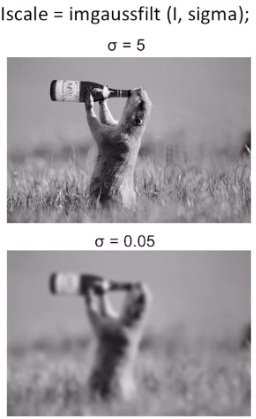
\includegraphics[scale=0.5]{1.png} 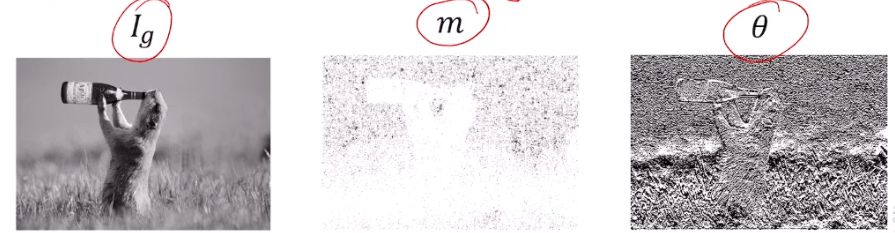
\includegraphics[scale=0.6]{2.png}
\end{center}
\pagebreak
\begin{list}{}{}
	\item[4.] Create \textbf{gradient histogram}\begin{list}{}{}
		\item 4$\times$4 gradient window
		\item Histogram of 4$\times$4 per window on 8 orientation bins
		\item Gaussian weighting on center keypoint (width = $1.5\sigma$)
		\item 4$\times$4$\times$8 = 128 descriptor size
	\end{list}
\end{list}
\begin{center}
	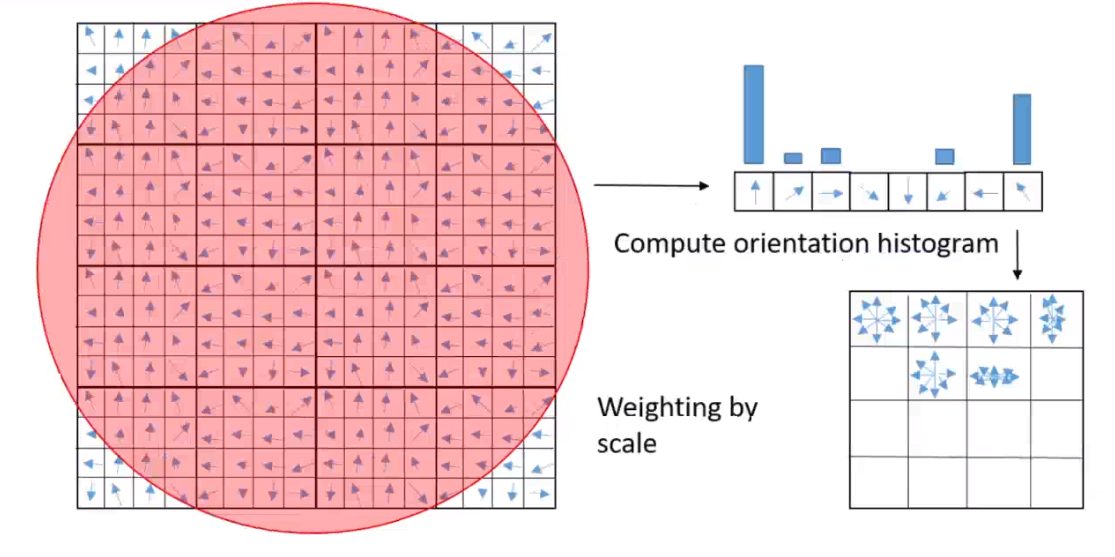
\includegraphics[scale=0.5]{3.png}
\end{center}
\subsubsection{Detectors}
\paragraph{Visual Feature Detector} Properties
\begin{list}{}{}
	\item \textbf{Repeatability} Detect the same feature in different image portions and different images, under different conditions (color, luminance\ldots). So with respect to translation, photometric changes, rotation, scaling and affine transformations (non-isotropic changes, for example the relative position of the camera)\ldots
\end{list}
\paragraph{Edge Detection} We need to find interesting points, talking about fundamental elements, basic components. One possible example are the edges of the image.\\
Reasoning in changes of intensity: edges are those points where the intensity changes.\begin{center}
	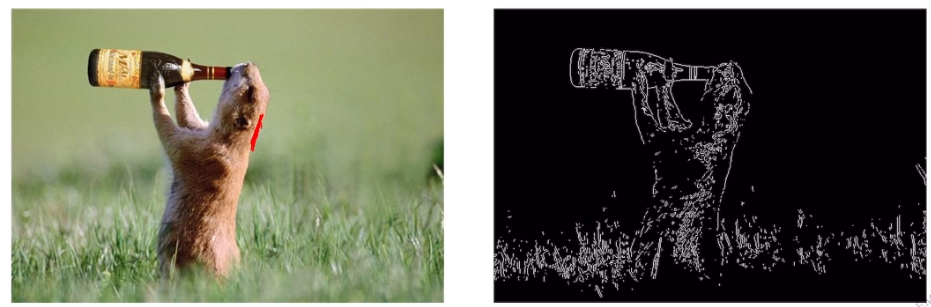
\includegraphics[scale=0.5]{4.png}
\end{center}
Typically using an edge detector filter on each pixel and turning pixels white or black by thresholding
\subparagraph{Edges and Gradients} The image gradient (graylevel) is $$\nabla I = \left[\frac{\partial I}{\partial x},\frac{\partial I}{\partial y}\right]$$ which is basically two images, gradient in both $x$ and $y$ directions. Edge are pixel regions where intensity gradient changes abruptly. The return of finite difference methods:
\begin{list}{}{}
	\item $G_x = \frac{\partial I}{\partial x} \simeq I(x+1,y)-I(x-1,y)$
	\item $G_y = \frac{\partial I}{\partial y} \simeq I(x,y+1)-I(x,y-1)$
\end{list}
\pagebreak
Edge detectors build on this idea combining with some smoothing: average on multiple pixels.
\subparagraph{Prewitt operators}
$$G_x = \left[\begin{array}{c c c }
+1&0&-1\\
+1&0&-1\\
+1&0&-1
\end{array}\right]\:\:\:\:\:G_y = \left[\begin{array}{c c c }
+1&+1&+1\\
0&0&0\\
-1&-1&-1
\end{array}\right]$$
\begin{center}
	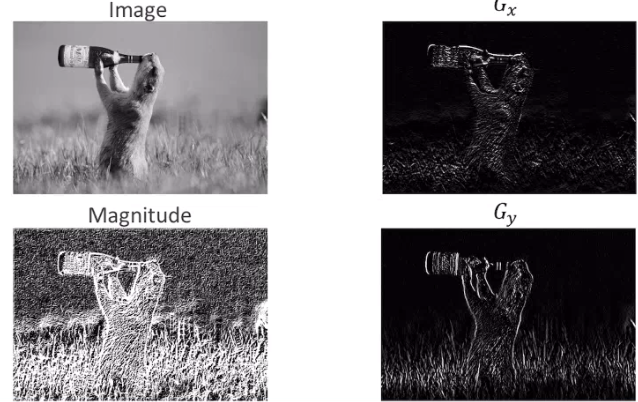
\includegraphics[scale=0.5]{5.png}
\end{center}
\subparagraph{Sobel Operator}
$$G_x = \left[\begin{array}{c c c }
+1&0&-1\\
+2&0&-2\\
+1&0&-1
\end{array}\right]\:\:\:\:\:G_y = \left[\begin{array}{c c c }
+1&+2&+1\\
0&0&0\\
-1&-2&-1
\end{array}\right]$$
Often with a constant $c\simeq \frac{1}{8}$ for scaling.
\begin{center}
	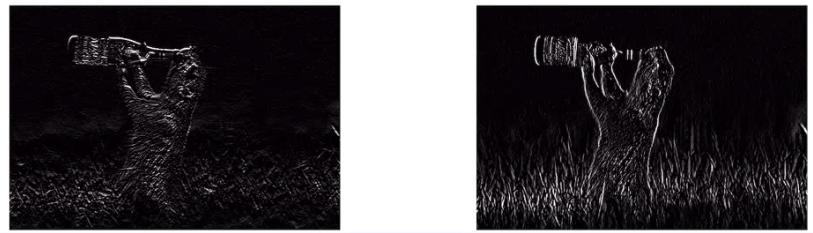
\includegraphics[scale=0.4]{6.png}
\end{center}
\paragraph{Blob Detection} Pixel regions with little gradient variability.\\
$g_\sigma(x,y)$ has maximum response when centered on a circle of radius $\sqrt{2}\sigma$, with $\sigma$ being the scale of the gaussian.\\
Laplace of Gaussian (LoG):
$$\nabla^2g_\sigma(x,y)=\frac{\partial^2g_\sigma}{\partial x^2} + \frac{\partial^2g_\sigma}{\partial y^2}$$
Typically using a scale normalized response
$$\nabla^2_{norm}g_\sigma(x,y)=\sigma^2\left(\frac{\partial^2g_\sigma}{\partial x^2} + \frac{\partial^2g_\sigma}{\partial y^2}\right)$$
\begin{enumerate}
	\item Convolve image with a LoG filter at different scales $\sigma = k\sigma_0$ by varying $k$ with a starting $\sigma_0$
	\item Find maxima of squared LoG responses:
	\begin{list}{}{}
		\item Find maxima on space-scale: focus on a scale and find maxima
		\item Find maxima between scales: do the same for all the scales and pick the maxima
		\item Threshold
	\end{list}
\end{enumerate}
The LoG can be approximated by the Difference of Gaussians (DoG) for efficiency, so to reuse part of the computations.
$$g_{k\sigma_0}(x,y) - g_{\sigma_0}(x,y) \simeq (k-1)\sigma_0^2\nabla^2g_{(k-1)\sigma_0}$$
SIFT uses LoG.
\paragraph{Affine Detectors} Laplacia-based detectors are invariant to scale thanks to the maximization in scale-space. Still not invariant to affine-transformation.
\begin{center}
	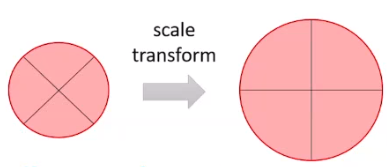
\includegraphics[scale=0.5]{7.png}\\
	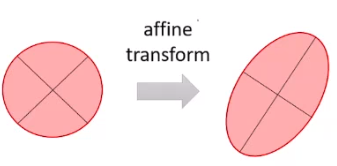
\includegraphics[scale=0.5]{8.png}
\end{center}
\paragraph{MSER} Maximally Stable Extremal Regions\\
Extract covariant regions (blobs) that are stable connected components of intensity sets of the image. Interesting areas stay the same at different thresholds: stable with respect to variations in luminance, not scale dependent and doesn't assume circular regions. The key idea is to \textbf{take the blobs} (\textbf{extremal regions}) \textbf{which are nearly the same through a wide range of intensity thresholds}.\\
Blobs are generated (locally) by binarizing the image over a large number of thresholds:\begin{list}{}{}
	\item Invariance to affine transformation of image intensities
	\item Stability (they are stable on multiple thresholds)
	\item Multi-scale (connected components are identified by intensity stability not by scale)
	\item Sensitive to local lightning effects, shadows\ldots
\end{list}
\subparagraph{Intuitions on MSER} Generate frames from the image by thresholding it on all graylevels.\\
Capture those regions that from a small seed of pixel grow to a stably connected region. Stability is assessed by looking at derivatives of region masks in time (most stable $\Rightarrow$ minima of connected region variation).
\paragraph{Image Segmentation} The process of partitioning an image into a set of homogeneous pixels, hoping to match objects or their subparts.\\
A naive approach: straighten the image in a $N\cdot M$ vector and use it as a dataset for K-means.\\
\subparagraph{Ncut} Normalized cuts
\begin{center}
	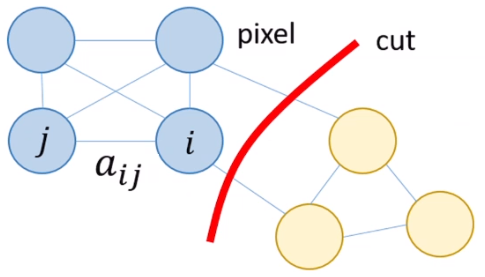
\includegraphics[scale=0.5]{9.png}
\end{center}
With each node being a pixel: an image is a graph. $a_{ij}$ is the affinity between pixels at a certain scale $\sigma$. A cut of $G$ is the set of edges such whose removal makes $G$ a disconnected graph. Breaking the graph into pieces by cutting edges of low affinity.\\
The normalized cut problem is NP-hard, approximate solution as an eigenvalue problem. But the eigenvalue decomposition it's really intractable with big images. We need to reduce the number of pixels. We can use \textbf{superpixels}: clustering the pixels with K-means (perhaps with different $K$) and using the clusters as nodes for segmentation algorithms (Ncut, Markov Random Fields\ldots). We can do multiscale superpixeling and segmenting at different scales, different policies\ldots\\
\subsubsection{Conclusion}
Image processing is a lot about convolutions: linear masks to perform gradient operations, gaussian functions to apply scale changes (zooming in and out). Computational efficiency is a driving factor: convolution in Fourier domain, superpixel, lightweight feature detectors\ldots
\subsection{Wavelets}
\paragraph{Limitations of DFT} Sometimes we might need localized frequencies rather than global frequency analysis.
\begin{center}
	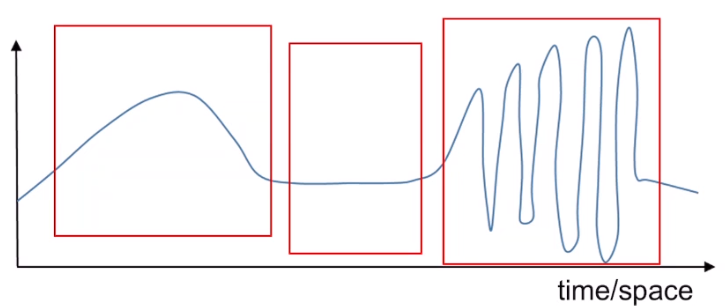
\includegraphics[scale=0.5]{10.png}
\end{center}
We slice the signal in "time slots" in time analysis and "frequency slots" in frequency analysis. In wavelet analysis you do both.\begin{center}
	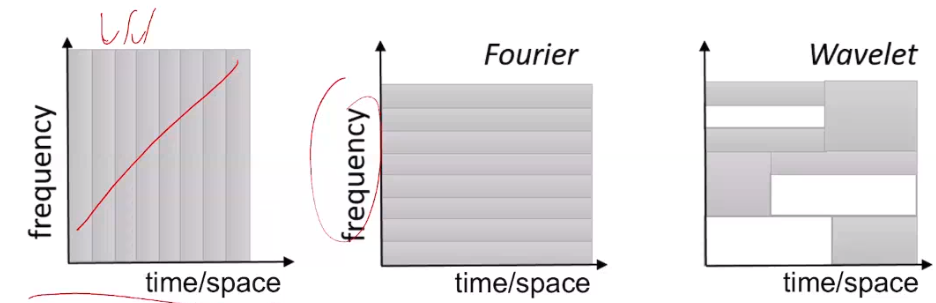
\includegraphics[scale=0.33]{11.png}\\
	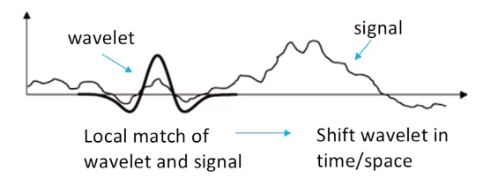
\includegraphics[scale=0.5]{12.png}
\end{center}
\begin{enumerate}
	\item Scale and shift original signal
	\item Compare signal to a wavelet
	\item Compute coefficient of similarity
\end{enumerate}
Split the signal with an orthonormal basis generate by translation and dilation of a mother wavelet $$\sum_t \hbox{x}(t)\phi_{j,k}(t)$$
Terms $k,j$ regulate scaling and shifting of the wavelet
$$\phi_{t,k}(\hbox{x}) = 2^{\frac{k}{2}}\phi\left(\frac{t-j2^k}{2^k}\right)$$
With many different options for the mother wavelet $\phi$
\begin{center}
	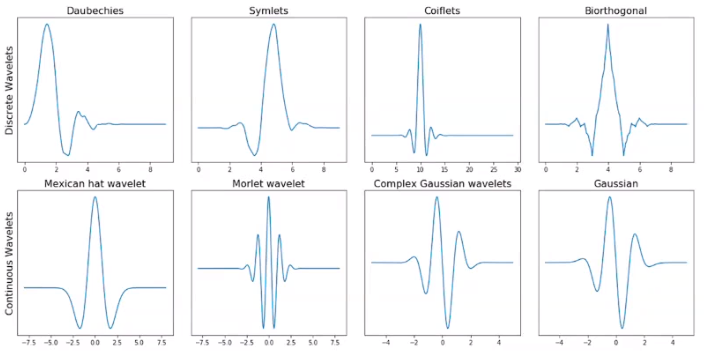
\includegraphics[scale=0.5]{13.png}
\end{center}
Scaling and dilation is akin to a sort of frequency: high scale mean stretched wavelet with slowly changing coarse feature and low frequency, while low scale compressed wavelet with rapidly changing details and high frequency.
\paragraph{DWT} Discrete Wavelet Transform: uses a finite set of scales and shifts rather than "any possible value" as in the continuous wavelet transform.
\section{Generative and Graphical Models}
Generative referring to the probability we learn: if we know the distribution probability of data we can generate new data.\\
Graphical referring to graphical formalisms that describe in a syntetic way the structures we'll see.
\paragraph{Generative Learning} ML models that represent knowledge inferred from data under the form of probabilities:
\begin{list}{}{}
	\item Probabilities can be sample: new data can be generated
	\item Supervised, unsupervised, weakly supervised tasks
	\item More easily incorporate prior knowledge on data and tasks
	\item Interpretable knowledge (how data is generated)
\end{list}
The majority of modern tasks comprises large number of variables\begin{list}{}{}
	\item Modeling the joint distribution of all variables can become impractical
	\item Exponential size of the parameter space
	\item Computationally impractical to train and predict
\end{list}
\paragraph{Representation} Graphical models are a compact way to represent exponentially large probability distributions. Encode conditional independence assumptions, and different classes of graph structures imply different assumptions/capabilities.
\paragraph{Inference} How to query (predict with) a graphical model? Probability of unknown $X$ given observations $d$, $P(X\:|\:d)$, the \textbf{most likely hypothesis} (parameters) $X$.
\paragraph{Learning} Find the right model parameters.
\paragraph{Representation} A graph whose nodes are random variables and edges represent probabilistic relationships between the variables.\\
Different classes of graphs:
\begin{list}{}{}
	\item Directed edges express \textbf{causal relationships}
	\item Undirected edges express \textbf{soft constraints}, values cannot change independently
	\item \textbf{Dynamic models}, graphs subject to structure changes to reflect dynamic processes. For example RNNs: recurrent neural networks are unfolded using weight sharing, producing a dynamic model.
\end{list}
\paragraph{In Deep Learning} Bayesian learning necessary to understand Variational Deep Learning.
\begin{center}
	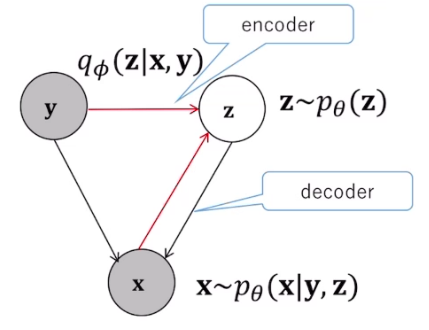
\includegraphics[scale=0.5]{14.png}
\end{center}
\paragraph{Generate new knowledge} Complex data can be generated if the model is powerful enough to capture its distribution.
\subsection{Probability Refresher}
\texttt{todo}
\subsubsection{Inference} Bayesian: consider all hypothesis weighted by their probabilities
$$P(X\:|\:d)=\sum_i P(X\:|\:h_i)P(h_i\:|\:d)$$
MAP (Maximum a-Posteriori): infer $X$ from $P(X\:|\:h_{MAP})$ where $h_{MAP}$ is the maximum a-posteriori hypothesys given $d$
$$h_{MAP} = \arg\max_{h\in H} P(h\:|\:d) = \arg\max_{h\in H} P(d\:|\:h)P(h)$$
ML assuming uniform prioris $P(h_i)=P(h_j)$ yields the maximum likelihood (ML) estimate $P(X\:|\:h_{ML})$ $$h_{ML} = \arg\max_{h\in H} P(d\:|\:h)$$
Any probability can be obtained from the Joint Probability Distribution $P(X_1,\ldots,X_n)$ by marginalization but at an exponential cost (e.g. $2^{n-1}$ for a marginal distribution from binary RV)
\subsection{Graphical Models}
Compact graphical representation for exponentially large joint distributions: simplifies marginalization and inference algorithms, allowing to \textbf{incorporate prior knowledge} concerning causal relationships and associations between random variables.\begin{list}{}{}
	\item Directed graphical models (Bayesian Networks)
	\item Undirected graphical models (Markov Random Fields)
\end{list}
\subsubsection{Bayesian Networks} 
\begin{multicols}{2}
Directed Acyclic Graphs (DAG) $G = (V,E)$\begin{list}{}{}
	\item Nodes $v\in V$ represent random variables\\
	Shaded $\Rightarrow$ observed, empty (like $Y_3$) $\Rightarrow$ unobserved
	\item Edges $e\in E$ describe the conditional independence relationships
\end{list}
\columnbreak
\begin{center}
	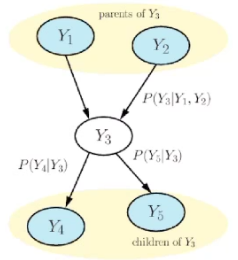
\includegraphics[scale=0.5]{15.png}
\end{center}
\end{multicols}
\paragraph{Conditional Probability Tables} CPTs are local to each node and describe the probability distribution \textbf{given its parents}.
$$P(Y_1,\ldots,Y_n) = \prod_{i=1}^N P(Y_i\:|\:\hbox{Parents}(Y_i))$$
\paragraph{Plate notation} If the same causal relationship is replicated for a number of variables, we can compactly represent it with plate notation.
$$P(Y_1,\ldots,Y_N,C) = P(C)\prod_{i=1}^N P(Y_i\:|\:C)$$
\begin{center}
	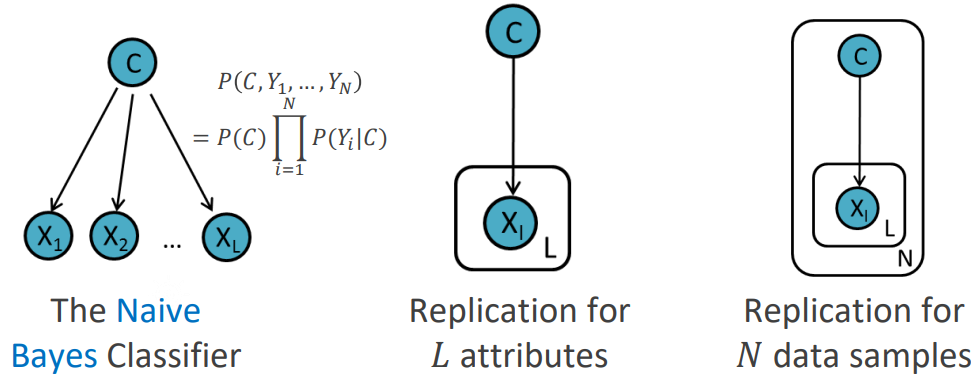
\includegraphics[scale=0.5]{16.png}
\end{center}
\paragraph{Full-Plate Notation}
Boxes denote replication for a number of times (denoted by the letter in the corner). Shaded nodes are observed variables, empty nodes are unobserved latent variables.\\
Black dots (optional) identify model parameters.
\begin{center}
	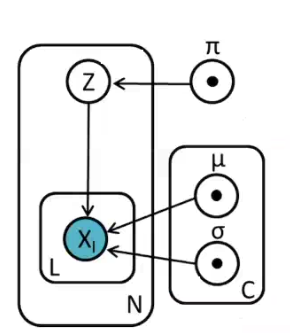
\includegraphics[scale=0.5]{17.png}
\end{center}
\subsubsection{Markov Random Fields}
\begin{center}
	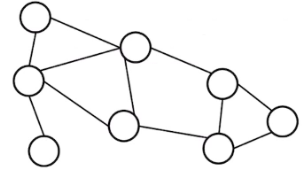
\includegraphics[scale=0.5]{18.png}
\end{center}
Undirected graph $G = (V,E)$ (a.k.a. Markov Networks). Also with shaded/empty nodes to denote observed/unobserved variables.\\
Edges $e\in E$ represent bidirectional dependencies between variables (constraints).\\
Often arranged in a structure that is coherent with the data/constraint we want to model.\\
Often used in image processing to impose spatial constraints (e.g. smoothness)
\subsection{Conditional Independence and Causality}
Can we reason on the structure of the graph to infer direct/indirect relationships between random variables?
\paragraph{Local Markov Property} Each node (random variable) is conditionally independent of all its non-descendants given a joint state of its parents. $$Y_v\perp Y_{V\setminus \hbox{Children(v)}}\hbox{ given }Y_{\hbox{Parent}(v)}\:\:\forall\:v\in V$$
There are substructures in the Bayesian networks with which we can build everything.
\paragraph{Markov Blanket} A Markov blanket $Mb(A)$ of a node $A$ is the minimal set of vertices that isolates/shields the node from the rest of the Bayesian network. If I know the variables in $Mb(A)$ then I know everything I need to know about $A$\begin{center}
	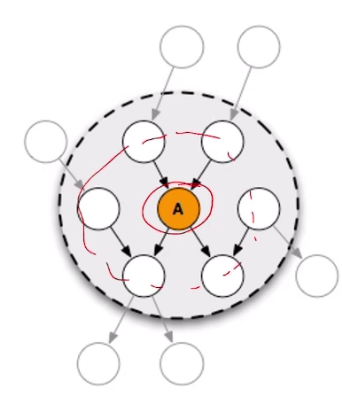
\includegraphics[scale=0.5]{19.png}
\end{center}
Taking only the parents it's not sufficient, we need also the children and the co-parents (nodes that are parents of one of my children). So it contains parents, children and children's parents.
$$P(A\:|\:Mb(A), Z) = P(A\:|\:Mb(A))\:\:\forall\:Z\not\in Mb(A)$$
\paragraph{Joint Probability Factorization} An application of the chain rule and local Markov property.\begin{enumerate}
	\item Pick a topological ordering of the nodes
	\item Apply chain rule following the order
\end{enumerate}
\paragraph{Sampling of a Bayesian Network} A BN describes a generative process for observations.
\begin{enumerate}
	\item Pick a topological ordering of the nodes
	\item Generate data by sampling from the local condition probabilities following this order
\end{enumerate}
Generate $i$th sample for each variable, example $s_i\simeq P(S)$, $h_i\simeq P(H\:|\:S=s_i)$
\subsection{Fundamental Bayesian Network Structures}
Three fundamental substructures that determine the conditional independence relationships in a Bayesian network.
\paragraph{Tail to Tail} Common cause \begin{center}
	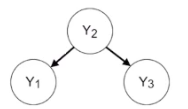
\includegraphics[scale=0.75]{20.png}
\end{center}
$$P(Y_1,Y_3\:|\:Y_2)=P(Y_1\:|\:Y_2)P(Y_3\:|\:Y_2)$$
If $Y_2$ is unobserved, then $Y_1,Y_3$ are marginally dependent $Y_1\not\perp Y_3$\\
If $Y_2$ is observed, $Y_1,Y_3$ become conditionally independent $Y_1\perp Y_3\:|\:Y_2$ (the path between $Y_1,Y_3$ is blocked by the observed (shaded) $Y_2$)
\paragraph{Head to Tail} Causal Effect \begin{center}
	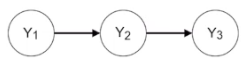
\includegraphics[scale=0.75]{21.png}
\end{center}
$$P(Y_1,Y_3\:|\:Y_2)=P(Y_1)P(Y_2\:|\:Y_1)P(Y_3\:|\:Y_2)=P(Y_1\:|\:Y_2)P(Y_3\:|\:Y_2)$$
Same behavior as before!\\
If $Y_2$ is unobserved, then $Y_1,Y_3$ are marginally dependent $Y_1\not\perp Y_3$\\
If $Y_2$ is observed, $Y_1,Y_3$ become conditionally independent $Y_1\perp Y_3\:|\:Y_2$ ($Y_2$ again blocks the path)
\paragraph{Heat to Head} Common effect\begin{center}
	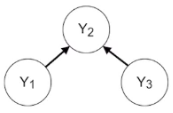
\includegraphics[scale=0.75]{22.png}
\end{center}
$$P(Y_1,Y_2,Y_3) = P(Y_1)P(Y_3)P(Y_2\:|\:Y_1,Y_3)$$
If $Y_2$ is unobserved, then $Y_1,Y_3$ are marginally independent $Y_1\perp Y_3$\\
If $Y_2$ is observed, then $Y_1,Y_3$ are conditionally dependent $Y_1\not\perp Y_3\:|\:Y_2$\\
If any $Y_2$ descendants is observed it unlocks the path.
\paragraph{Derived Conditional Independence Relationships} A Bayesian network represent the local relationship encoded by the 3 basic structures plus the derived relationships.\\\\
Given the same distribution I can have two different Bayesian Networks, which implies the same factorization.
\begin{center}
	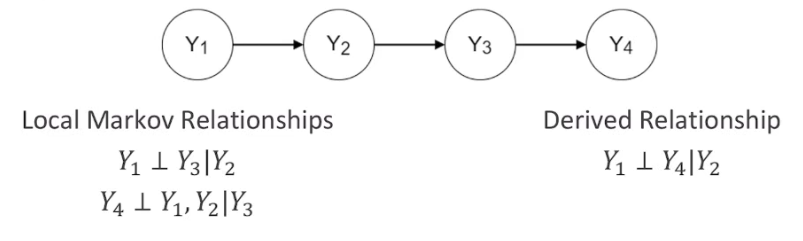
\includegraphics[scale=0.5]{23.png}
\end{center}
\paragraph{$d$-separation} Let $r = Y_1\leftrightarrow\ldots\leftrightarrow Y_2$ be an undirected path between $Y_1,Y_2$, $r$ is $d$-separated by $Z$ if there exist at least one node $Y_c\in Z$ for which path $r$ is blocked. With $Z$ being the set of variable for which we're assessing this separation.\\
In other words, this holds if at least one of the following holds:\begin{list}{}{}
	\item $r$ contains an head-to-tail structure $Y_i\rightarrow Y_c\rightarrow Y_j$ (or $Y_i\leftarrow Y_c\leftarrow Y_j$) and $Y_c \in Z$
	\item $r$ contains a tail-to-tail $Y_i\leftarrow Y_c\rightarrow Y_j$ and $Y_c \in Z$
	\item $r$ contains head-to-head $Y_i\rightarrow Y_c\leftarrow Y_j$ and neither $Y_c$ nor its descendants are in $Z$
\end{list}
Two nodes $Y_i,Y_j$ in a Bayesian Network $G$ are $d$-separated by $Z\subset V$ $\Leftrightarrow$ all undirected paths between $Y_i,Y_j$ are $d$-separated by $Z$ (denoted by $\hbox{Dsep}_G(Y_i,Y_j\:|\:Z)$)
\paragraph{Markov Blanket} The Markov Blanket $Mb(Y)$ is the minimal set of nodes which $d$-separates a node $Y$ from all other nodes (i.e. makes $Y$ conditionally independent of all other nodes in the Bayesian Network)
$$Mb(Y) = \{\hbox{Parents}(Y), \hbox{Children}(Y), \hbox{Parents}(\hbox{Children}(Y))\}$$
\paragraph{Are Directed Models Enough?} Bayesian Networks are used to model asymmetric dependencies. But Directed Models cannot express all conditional dependence relationships: expressing some precludes the expressions of others.\\
What if we want to model symmetric dependencies: bidirectional effects, spatial dependencies... we need \textbf{undirected approaches}. Directed models cannot represent some bidirectional dependencies in the distributions.
\subsection{Markov Random Fields}\begin{center}
	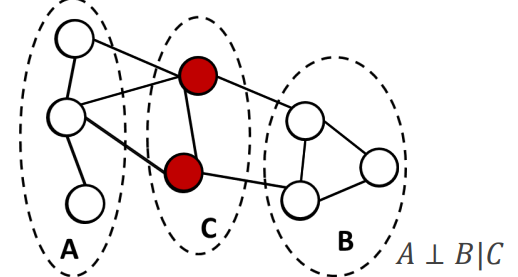
\includegraphics[scale=0.5]{24.png}
\end{center}
What is the undirected equivalent of $d$-separation in directed models? It's based on node separation: the two nodes in the middle separate the two lateral parts.\\
Node subsets $A,B\subset V$ are conditionally independent given $C\subset V\setminus \{A,B\}$ if all paths between nodes in $A$ and $B$ pass through at least one of the nodes in $C$.\\
The Markov Blanket of a node includes all and only its neighbors.
\paragraph{Joint Probability Factorization} What is the undirected equivalent? We seek a product of functions defined over a set of nodes associated with some local properties of the graph. Markov blanket tells that nodes that are not neighbors are conditionally independent given the remainder of the nodes.$$P(X_v,X_i\:|\:X_{V\setminus\{v,i\}}) = P(X_v\:|\:X_{V\setminus\{v,i\}})P(X_i\:|\:X_{V\setminus\{v,i\}})$$
Factorization should be chosen in a way that nodes $X_v$ and $X_i$ are not in the same factor: we use a well-known graph structure that includes only nodes that are pairwise connected.
\subparagraph{Clique} Subset of nodes $C$ in graph $G$ such that $G$ contains an edge between all pair of nodes in $C$. It's maximal if you cannot add more nodes.
\subparagraph{Maximal Clique Factorization} Define $X = X_1,\ldots,X_n$ as the random variables associated to the $N$ nodes of the undirected graph $G$ $$P(X)=\frac{1}{Z}\prod_C \psi(X_C)$$
$X_C$ are the random variables in the maximal clique $C$, $\psi(X_C)$ is the \textbf{potential function} over the maximal clique $C$ and $Z$ is the partition function ensuring normalization.
$$Z = \sum_X\prod_C\psi(X_C)$$
The partition function $Z$ is the computational bottleneck of undirected modes: $O(K^N)$ for $N$ discrete random variables with $K$ distinct values.
\paragraph{Potential Functions} Potential functions $\psi(X_C)$ are not probabilities, they express which configuration of the local variables are preferred. For example $\psi(X_1,X_2)=\left\{ \begin{array}{l l}
1&\hbox{if }X_1 = X_2\\
4&\hbox{if }X_2 = 2X_1\\
0&\hbox{otherwise}
\end{array}\right.$: you can hand-engineer feature functions.\\
If we restrict to strictly positive potential functions, the Hammersley-Clifford theorem provides guarantees on the distribution that can be repreesented by the clique factorization.
\paragraph{Boltzmann Distribution} A convenient and widely used strictly positive representation of the potential function is $$\psi(X_C)=e^{-E(X_C)}$$
where $E(X_C)$ is called \textbf{energy function}.
\subsubsection{From Directed to Undirected}
Straightforward when is linear.\\Requires some work with v-structures, e.g. \textbf{moralization} (a.k.a. marrying of the parents).\begin{center}
	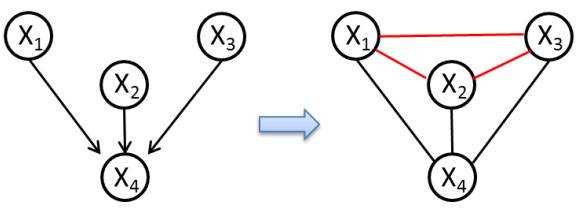
\includegraphics[scale=0.5]{25.png}
\end{center}
\subsection{Learning Causation from Data}
\paragraph{Learning with Bayesian Network}
\begin{center}
	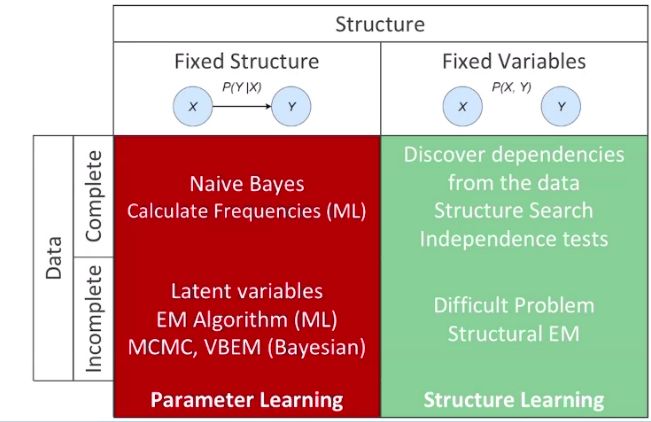
\includegraphics[scale=0.5]{26.png}
\end{center}
\paragraph{Structure Learning Problem} Observations are given for a set of fixed random variables, and network structure is not specified:\begin{list}{}{}
	\item Determine which arcs exist in the network (causal relationships)
	\item Compute Bayesian network parameters (conditional probability tables)
\end{list}
Determining causal relationships between variables entails deciding on arc presence and directing edges.
\subparagraph{Structure Finding Approaches}\begin{list}{}{}
	\item \textbf{Search and Score}\\A model selection approach, a search in the space of the graphs.\\
	Search the space Graph$(Y)$ of graphs $G_k$ that can be built on the random variables $Y = Y_1,\ldots,Y_N$, scoring each structure by $S(G_k)$ and returning the highest scoring graph $G^*$. So two fundamental aspects: the scoring function and the search strategy.\\
	\textbf{Scoring function}: two fundamental properties:\begin{list}{}{}
		\item Consistency: same score for graphs in the same equivalence class
		\item Decomposability: can be locally computed
	\end{list}
	Two approaches:\begin{list}{}{}
		\item Information theoretic: based on data likelihood plus some model-complexity penalization terms
		\item Bayesian: score the structures using a graph posterior (likelihood plus proper prior choice
	\end{list}
	\textbf{Search strategy}:\begin{list}{}{}
		\item Finding maximal scoring structures is NP complete
		\item Constrain search strategy: starting from a candidate structure we modify iteratively by local operations (edge/node addition/deletion). Each operation has a cost, so a cost optimization problem.
	\end{list}
	Constrain search space can be\begin{list}{}{}
		\item Known node order: can reduce the search space to the parents of each node (Markov Blankets)
		\item Search in the space of structure equivalence classes
		\item Search in the space of node ordering
	\end{list}
	\item \textbf{Constraint Based}\\
	Tests of conditional independence $I(X_i,X_j\:|\:Z)$, constraining the network. Based on measures of association between two variables $X_i$ and $X_j$ given their neighbor nodes $Z$.\\
	\textbf{Testing strategy}:\begin{list}{}{}
		\item Choice of the testing order is fundamental in avoiding a super-exponential complexity.
		\item Level-wise testing: tests $I(X_i,X_j\:|\:Z)$ are performed in order of increasing size of the conditioning set $Z$ starting from $Z = \emptyset$ (PC algorithm)
		\item Node-wise testing: tests are performed on a single edge at the time, exhausting independence checks on all conditioning variables (TPDA algorithm)
		\item The nodes entering $Z$ are chosen in the neighborhood of $X_i,X_j$
	\end{list}
	\item \textbf{Hybrid}\\
	Model selection of constrained structures. Multi-stage algorithm combining previous approaches: independence tests to find a good sub-optimal skeleton as starting point, then search and score refining the skeleton.\\
	Max-Min Hill Climbing (MMHC) model: optimized constraint-based approach to reconstruct the skeleton, using the candidate parents in the skeleton to run a search and score approach.
\end{list}
\subsection{Hidden Markov Models}
\paragraph{Sequence}A sequence $y$ is a collection of observations $y_t$ where $t$ represent the position of the element according to a complete order (e.g. time)
$$y_1\rightarrow \ldots\rightarrow y_{t-1}\rightarrow y_t\rightarrow\ldots\rightarrow y_T$$
$$P(y_t\:|\:y_{t-1})$$
Also head-to-tail: observation at time $t$ is independent from $t=1,\ldots,t-1$: \textbf{first-order Markov assumption}.\\
Reference population is a set of independent and identically distributed sequences $y^1, \ldots, y^N$\\
Difference sequences generally have different lengths $T^1,\ldots,T^N$
\paragraph{Markov Chain} First-Order Markov Chain is a directed graphical model for sequences such that element $x_t$ only depends on the $t-1$ previous nodes.\\
We have X = $x-1,\ldots,x_T$ that can be represented as 
$$x_1\rightarrow \ldots\rightarrow x_{t-1}\rightarrow x_t\rightarrow\ldots\rightarrow x_T$$
So we can write $$P(\hbox{X}) = P(x_1,\ldots,x_T) = P(x_1)\cdot\prod_{i=2}^T P(x_i\:|\:x_{i-1})$$
because $P(x_i\:|\:x_{i-1})$ is the same whenever the $t$.\\
$P(x_1)$ is the \textbf{prior distribution} ($x_1$ has nothing "before" it) and $P(x_i\:|\:x_{i-1})$ is the \textbf{transition distribution}.\\\\
If I assume $x_t\in\{a,\ldots,z\}$, so of 25 elements, this gives $P(x_1) = P(x_1 =$ letter$)$ so $P(x_1)$ is a vector with each position being the probability of $x_1$ being that letter. Summing the vector elements gives 1, because it's a distribution of probabilities.\\
$P(x_i\:|\:x_{i-1})$ is a 25$\times$25 matrix: in position $n,b$ is $P(x_i=n\:|\:x_{i-1}=b)$. The elements in a single column will give $1$, because conditional probability gives a family of distribution: for each assignment I have a distribution.\\\\
The general form is the $L$th order Markov chain, when $x_i$ depends on $L$ predecessors.
\paragraph{Observed Markov Chains} We can use the Markov chain to model the relationships between observed elements in a sequence. The problem is that we can do that only pairwise: computational issue (very large matrices) and e.g. only co-occurrence of 2 words so unapplicable to natural language.\\
So we need to abstract from symbols to category: not relationship between words, but relationships between the general concepts represented by those words. The categories are not observable: Markov chain over non-observable elements.
\paragraph{Hidden Markov Models} HMM infer categories: stochastic process where transition dynamics is disentangles from observations generated by the process.\begin{center}
	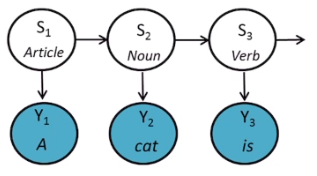
\includegraphics[scale=0.5]{27.png}
\end{center}
$S_i$ are \textbf{hidden states}, finite $i = 1,\ldots,C$.\\
We need \textbf{clustering algorithms}: clustering symbols into a finite set of non-observable elements.\\
Multinomial state transition
$$A_{ij} = P(S_t=i\:|\:S_{t-1}=j)$$
Prior probability (\textbf{stationary assumption})
$$\pi_i = P(S_1=i)$$
\textbf{Emission distribution} (the "down arrow" $\begin{array}{c}
S_t\\\downarrow\\Y_t
\end{array}$)
$$b_i(y_t) = P(Y_t = y_t\:|\:S_t = i)$$
\paragraph{HMM Joint Probability Factorization} Discrete state HMMs are parameterized by the finite number of hidden states $C$ and $\Theta = (\pi, A, B)$:
\begin{list}{}{}
	\item $\pi$ prior distribution
	\item $A$ state transition
	\item $B$ emission distribution (or its parameters)
\end{list}
$$P(Y = y) = \sum_s P(Y=y,S=s) =$$
$$= \sum_{s_1,\ldots,s_T}\left( P(S_1=s_1)P(Y_1=y_1\:|\:S_1=s_1)\prod_{t=2}^T P(S_t=s_t\:|\:S_{t-1} = s_{t-1})P(Y_t=y_t\:|\:S_t=s_t)\right)$$
\paragraph{HMMs as Recursive Models} A graphical framework describing how contextual information is recursiverly encoded by both probabilistic and neural models.
\begin{center}
	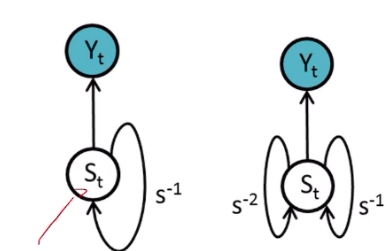
\includegraphics[scale=0.5]{28.png}
\end{center}
Indicates that the hidden state $S_t$ at time $t$ is dependent on context information from
\begin{list}{}{}
	\item the previous timestep $s^{-1}$, first-order
	\item the previous two timesteps $s^{-1},s^{-2}$, second-order
\end{list}
and so on.
\paragraph{HMMs as Automata} Can also be generalized to transducers.
\begin{center}
	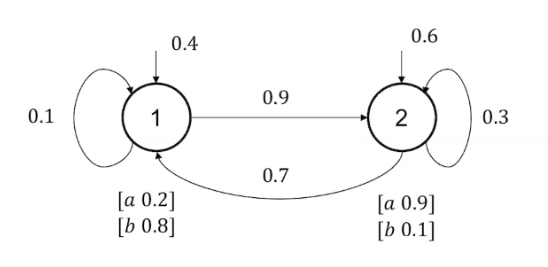
\includegraphics[scale=0.5]{29.png}
\end{center}
\pagebreak
\subsection{Notable Inference Problems}
\paragraph{Smoothing} Given a model $\Theta$ and an observed sequence $y$, determine the distribution of the hidden state at time $t$: $P(S_t\:|\:Y=y,\Theta)$\\
Forward Backward algorithm.
\paragraph{Learning} Given a dataset of $N$ sequences $D=\{y^1,\ldots,y^N\}$ and the number of hidden states $C$, find the parameters $\pi,A,B$ that maximize the probability model $\Theta = \{\pi,A,B\}$ having generated the sequences in $D$
\paragraph{Optimal State Assigment} Given a model $\Theta$ and an observed sequence $y$, find an optimal state assignment $s = s_1^*,\ldots,s_T^*$ for the hidden Markov chain.\\
Viterbi algorithm.
\subsubsection{Forward-Backward Algorithm} \textbf{Smoothing}: how do we determine $P(S_t = i\:|\:\hat{y})$? We will compute $P(S_t=i, \hat{y})$, it's proportional (just divide by $P(\hat{y})$).\\
I know $\Theta$, the model (its parameters). So I know $P(S_1) = \pi, P(S_t\:|\:S_{t-1} = A$ and $P(y_t\:|\:S_t) = B$: I need to express the quantity I want in terms of $\Theta=\{\pi,A,B\}$.\\
$\hat{y}$ are all the observations for each timestep $\Rightarrow P(S_t=i,y_1,\ldots,y_{t-1},y_t,y_{t+1},\ldots,y_T)$
$$\begin{array}{ccccccccccccc}
S_1&\rightarrow&\ldots&\rightarrow&S_{t-1}&\rightarrow&S_t&\rightarrow&S_{t+1}&\rightarrow&\ldots&\rightarrow&S_T\\
\downarrow& &\ldots& &\downarrow& &\downarrow& &\downarrow& &\ldots& &\downarrow\\
y_1&\rightarrow&\ldots&\rightarrow&y_{t-1}&\rightarrow&y_t&\rightarrow&y_{t+1}&\rightarrow&\ldots&\rightarrow&y_T
\end{array}$$
We are at time $t$, so everything after that is the future ($y_{t+1:T}$), and everything up to $t$ included is the past ($y_{1:t}$).
$$P(S_t=i,y_1,\ldots,y_{t-1},y_t,y_{t+1},\ldots,y_T) = P(y_{t+1:T}\:|\:S_t=i, y_{1:t}) P(S_t=i,y_{1:t})$$
If I observe $S_t$ we block the path $y_{1:t}$, so $P(y_{t+1:T}\:|\:S_t=i, y_{1:t}) = P(y_{t+1:T}\:|\:S_t=i)$
$$P(S_t=i,y_1,\ldots,y_{t-1},y_t,y_{t+1},\ldots,y_T) = P(y_{t+1:T}\:|\:S_t=i) P(S_t=i,y_{1:t})$$
I can derive two "messages"
\begin{list}{}{}
	\item Past message $\alpha_t(i) = P(S_t=i,y_{1:t})$ (\textbf{forward recursion})
	\item Future message $\beta_t(i) = P(y_{t+1:T}\:|\:S_t=i)$ (\textbf{backward recursion})
\end{list}
$$P(S_t,y_{1:t}) = \sum_{j=1}^c P(S_t, S_{t-1}=j,y_{1:t}) = \sum_{j=1}^c P(y_t\:|\:S_t, S_{t-1} = j, y_{1:t-1})P(S_t,S_{t-1},y_{1:t-1})$$
But we can get rid of $S_{t-1}=j$ and $y_{1:t-1}$ leaving us with $P(y_t\:|\:S_t)$ which is just the emission.\\
The second factor can be rewrited as $P(S_t\:|\:S_{t-1}=j,y_{1:t-1}) P (S_{t-1}=j\:|\:y_{1:t-1})$ and observing $S_{t-1}$ allows us to get rid of $y_{1:t-1}$, giving us the transition distribution $P(S_t\:|\:S_{t-1}=j)$ and $\alpha_{t-1}(j)$
$$\alpha_t(i) = P(S_t=i,y_{1:t}) = \sum_{j=1}^c P(y_t\:|\:S_t=i) P(S_t=i\:|\:S_{t-1}=j)\alpha_{t-1}(j)$$
$$\alpha_1(j) = P(y_1\:|\:S_1=j)P(S_1=j)$$
This just by reasoning with conditional independence.\\
Same thing can be done for $$P(y_{t+1:T}\:|\:S_{t} = i) = \sum_j P(y_{t+1:T},S_{t+1}=j\:|\:S_t=i) = \sum_j P(y_{t+2:T}\:|\:S_t, S_{t+1},y_{t+1})P(S_{t+1},y_{t+1}\:|\:S_t=i)$$
Same as before, I can exclude $S_t, y_{t+1}$ because we observe $S_{t+1}$ so that factor is $\beta_{t+1}(j)$.\\
The second factor is rewritten as $P(S_{t+1}\:|\:S_t,y_{t+1})P(y_{t+1}\:|\:S_{t+1})$ which is the transition distribution (we can exclude $y_{t+1}$) times the emission distribution.
$$\beta_t(i) = \sum_j P(y_{t+1}\:|\:S_{t+1} = j)P(S_{t+1}=j\:|\:S_t=i)\beta_{t+1}(j)$$ %TODO check
$$\beta_T = 1$$
\paragraph{Sum-Product Message Passing} The Forward-Backward algorithm is an example of a sum-product message passing algorithm.\\
A forward recursion computing a generic message $\mu_\alpha$, backward recursion computing a generic message $\mu_\beta$\\
A general approach to efficiently perform exact inference in graphical models, with $\alpha_t \equiv \mu_\alpha(X_n)$ and $\beta_{t}\equiv \mu_\beta(X_n)$
$$\mu_\alpha(X_n) = \sum_{X_{n+1}} \psi(X_n, X_{n+1})\mu_\beta(X_{n+1})$$
\subsubsection{Learning in HMM}
Learning parameters $\Theta=(\pi,A,B)$ by \textbf{maximum} (log) \textbf{likelihood}
$$L(\Theta) = \log\prod_{n=1}^N P(Y^n\:|\:\Theta) = \log\prod_{n=1}^N\left(\sum_{S_1^n,\ldots,S_{T_n}^n} P(S_1^n)P(Y_1^n\:|\:S_1^n)\prod_{t=2}^T P(S_t^n\:|\:S_{t-1}^n)P(Y_t^n\:|\:S_t^n)\right)$$
Maximizing the joint likelihood of the sequences given the parameters considering them independent and identically distributed. We have to deal with the unobserved $S_t^n$ and the nasty sum in the log.\\
Expectation-Maximization of the \textbf{complete likelihood} $L_c(\Theta)$, optimizing a slightly different problem obtaining a not-reducing similar result. It's completed with indicator variables $z_{ti}^n=\left\{\begin{array}{c l}
1&\hbox{if }n\hbox{th chain is in state }i\hbox{ at time }t\\
0&\hbox{otherwise}
\end{array}\right.$ about the assignments $S_i^n$
\paragraph{Expectation-Maximization} Gives the red line: touching in the estimating point and not greater in the other points.
\begin{center}
	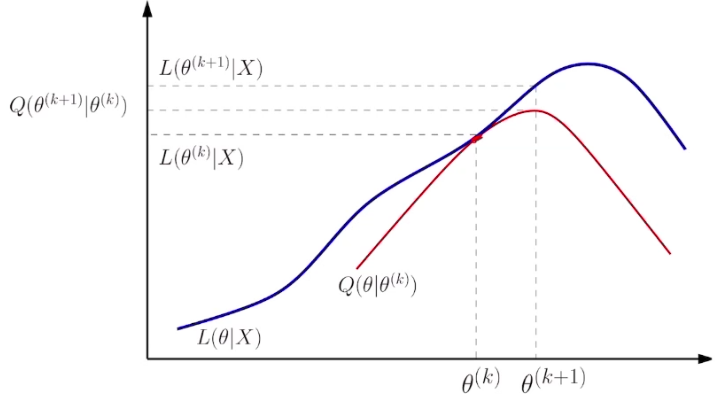
\includegraphics[scale=0.5]{30.png}
\end{center}
It's a matter of picking the right $Q(\Theta\:|\:\Theta^k)$\\
Introduce indicator variables in $L(\Theta)$ together with model parameters $\Theta = (\pi,A,B)$
$$L_C(\Theta)=\log P(X,Z\:|\:\Theta) = $$ %TODO formulona p.19 ISPR_7_HMM.pdf
But I built it assuming to know $z$, but I don't know it. The \textit{expectation} part is in this: I don't know $z_{ti}^n$, but you can optimize the function in expectation $E[L_C(\Theta)]$\\
It's a 2-step iterative algorithm for the maximization of complete likelihood $L_C(\Theta)$ with respect to the model parameters $\Theta$\begin{list}{}{}
	\item \textbf{E-step}: given the current estimate of the model parameters $\Theta^t$, compute $$Q^{t+1}(\Theta\:|\:\Theta^t) = E_{Z\:|\:X,\Theta^t}[\log P(X,Z\:|\:\Theta)]$$
	So compute the expectation of the complete log likelihood with respect to indicator variables $z_{ti}^n$ assuming estimated parameters $\Theta^t = (\pi^t, A^t, B^t)$ fixed at time $t$.\\
	Expectation with respect to a discrete random variable is $$E_z[Z] = \sum_z z\cdot P(Z=z)$$
	To compute the conditional expectation $Q^{t+1}(\Theta\:|\:\Theta^t)$ for the complete HMM log likelihood we need to estimate $$E_{Z\:|\:Y,\Theta^k}[z_{ti}] = P(S_t=i\:|\:y)$$
	$$E_{Z\:|\:Y,\Theta^k}[z_{ti}z_{(t-1)j}] = P(S_t = i, S_{t-1}=j\:|\:y)$$
	\pagebreak
	
	And we know how to compute the posteriors thanks to the forward-backward algorithm:
	$$y_t(i) = P(S_t = i\:|\:Y) = \frac{\alpha_t(i)\beta_t(i)}{\sum_{j=1}^C\alpha_t(j)\beta_t(j)}$$
	$$y_{t,t-1}(i,j) = P(S_t = i, S_{t-1} = j\:|\:Y) = \frac{\alpha_{t-1}(j)A_{ij}b_i(y_t)\beta_t(i)}{\sum_{m,l=1}^C \alpha_{t-1}(m)A_{lm}b_j(y_t)\beta_t(l)}$$
	\item \textbf{M-step}: find the new estimate of the model parameters $$\Theta^{t+1} = \arg\max_\Theta Q^{t+1}(\Theta\:|\:\Theta^t)$$
	Optimization problem, using the posteriors computed at the E-step. As usual with $$\frac{\partial Q^{t+1}(\Theta\:|\:\Theta^t)}{\partial\Theta}$$
	where $\Theta = (\pi, A, B)$ are now variables. The parameters can be distributions, so we need to preserve sum-to-one constraints (Lagrange Multipliers).\\
	State distributions are
	$$A_{ij}=\frac{\sum_{n=1}^N\sum_{t=2}^{T^n} \gamma_{t,t-1}^n(i,j)}{\sum_{n=1}^N\sum_{t=2}^{T^n}\gamma_{t-1}^n(j)}$$
	$$\pi_i=\frac{\sum_{n=1}^N\gamma_1^n(i)}{N}$$
	and the emission distribution, multinomial, is
	$$B_{ki} = \frac{\sum_{n=1}^N\sum_{t=1}^{T^n}\gamma_t^n(i)\delta(y_t=k)}{\sum_{n=1}^N\sum_{t=1}^{T^n}\gamma_t^n(i)}$$
\end{list}
With appropriate Lagrange multiplier is multinomial.
\paragraph{Usefulness of HMMs}\begin{list}{}{}
	\item \textbf{Regime Detection}: for example, you can only observe the volatility and you can model it according to a HMM that can capture it. For example with 2 states a model can be too simple, you can add hidden state (for example a 5-state HMM).\\
	The hidden states are \textbf{clustering the observations}.
\end{list}
\paragraph{Decoding Problem} Find the optimal state assignment s $= s_1^*,\ldots,s_T^*$ for an observed test sequence y given a trained HMM. No unique interpretation of the problem.\\
Can be done identifying the single hidden states $s_t$ that maximize the posterior $$s_t^*=\arg\max_{i=1,\ldots,C}P(S_t=i\:|\:Y)$$ 
or find the most likely \textbf{joint hidden state assignment} 
$$\hbox{s}^* = \arg\max_s P(Y,S = \hbox{s})$$
\paragraph{Viterbi Algorithm} Efficient dynamic programming algorithm based on a backward-forward recursion, example of max-product message passing algorithm. When exchanging, instead of $\sum$ we maximize the $\prod$.
%TODO check all
$$\max_{\hat{s} = s_1,\ldots,s_T} P(\hat{y},\hat{s}) = \max_{\hat{s}}\prod_{t=1}^T P(y_t\:|\:s_t)P(s_t\:|\:s_{t-1})$$
because is emission and prior as always. Let's focus on a simplified problem: first try to find the state that maximize $s_T$. Let's focus on $T$
$$\max_{s_T}\prod_{t=1}^T P(y_t\:|\:s_t)P(s_t\:|\:s_{t-1})=$$
we can exclude a lot
$$=\prod_{t=1}^{T-1} P(y_t\:|\:s_t)P(s_t\:|\:s_{t-1})\cdot\max_{s_T}P(y_T\:|\:s_T)P(s_T\:|\:s_{T-1})$$
which is a unique term, let's call $\epsilon(s_{T-1}) = \max_{s_T}P(y_T\:|\:s_T)P(s_T\:|\:s_{T-1})$, and $s_{T-1}$ has $c$ possible values, the number of hidden states.\\
So $\epsilon(s_{T-1})$ it's a vector of $c$ positions, and in position $j$ we have $\epsilon(s_{T-1} = j)$
$$\prod_t^{T-1} P(y_t\:|\:s_t)PSs_t\:|\:s_{t-1})\epsilon(s_{T-1})$$
Let's try solving 
$$\max_{s_{T-1}} \prod_t^{T-1} P(y_t\:|\:s_t)PSs_t\:|\:s_{t-1})\epsilon(s_{T-1})$$
we would do the same procedure. So we can iteratively start from the last item and use the information iteratively to compute the previous one.\\
In general we compute $$\epsilon(s_{t-1}) = \max_{s_t} P(y_t\:|\:s_t)P(s_t\:|\:s_{t-1})\epsilon(s_t)$$
So $s_t$ is received by $s_{t-1}$ to compute the new $\epsilon(s_{t-1})$ which is in turn passed to $s_{t-2}$ and so on, ending at the root. In practice we never choose the state, only computing the maximum. At the root, I have no predecessor states and can solve the maximization problem
$$s_1^* = \arg\max_{s_1}P(y_1\:|\:s_1)P(s_1)$$
From state $s_1$ we pick up $s_1^*$ and send it to $s_2$, which will use this information and pick the correct state that maximize the $\epsilon$.
\subsection{Input-output Hidden Markov Models}
\begin{center}
	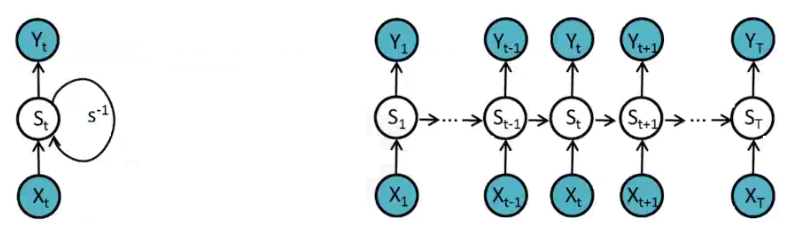
\includegraphics[scale=0.5]{31.png}
\end{center}
Translates an input sequence in an output sequence (\textbf{transduction}). State transition and emission depend on input observations (\textbf{input-driven}).\\
Recursive model highlights analogy with RNNs.
\paragraph{Bidirectional Input-Driven Models} Removes the causality assumption that current observation doesn't depend on the future and homogeneity assumption that a state transition doesn't depend on the position in the sequence.
\begin{center}
	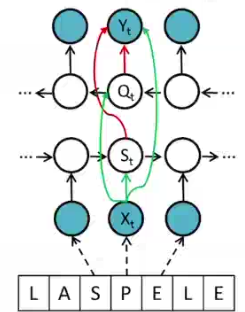
\includegraphics[scale=0.5]{33.png}
\end{center}
\paragraph{Coupled HMMs} Describing interacting processes whose observation follow different dynamics while the underlying generative processes are interlaced.
\begin{center}
	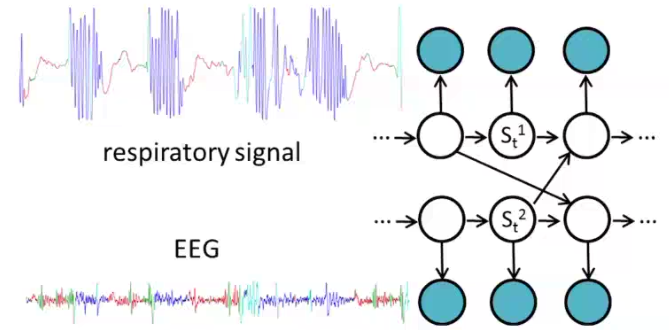
\includegraphics[scale=0.5]{32.png}
\end{center}
\paragraph{Dynamic Bayesian Networks} HMMs are a specific and the simples case of a class of directed models that represent dynamic processes and data with changing connectivity template. Other examples are: Hierarchical HMMs and structure changing information.\\
DBNs are graphical models whose structure changes to represent evolution across time and/or between different samples.
\subsection{Markov Random Fields}
MFRs are undirected graphs $G = (V, E)$. Nodes $v\in V$ are random variables $X_v$, edges $e\in E$ are bi-directional dependencies between variables.
\paragraph{Likelihood Factorization} Define X = $X_1,\ldots, X_N$ as the random variables associated to the $N$ nodes in the undirected graph $G$
$$P(\hbox{X}) = \frac{1}{Z}\prod_C \psi_C(X_C)$$\\
$X_C$ are the random variables associated to the maximal clique $C$, $\psi_C(X_C)$ is the \textbf{potential function} for clique $C$\\
With $Z$ normalization term used to transform to probability, from a \textbf{partition function}:
$$Z = \sum_X\prod_C\psi_C(X_C)$$
As already stated, potential functions are not probabilities, they express which configurations of the local variables are preferred. A conveniently and widely used strictly positive representation of the potential function is the \textbf{Boltzmann Distribution}:
$$\psi_C(X_C)=\exp\left(-E(X_C)\right)$$
with $E(X_C)$ called \textbf{energy function}.\\
In general we will assume to work with Markov Random Fields where the partition functions factorize as $$\psi_C(X_C) = \exp\left(-\sum_{k=1}^K\theta_{Ck}f_{Ck}(X_C)\right)$$
\begin{list}{}{}
	\item $K$ defines the number of feature functions that we use, so the cardinality of a dictionary of feature functions $f_{Ck}$
	\item $\theta_{Ck}\in R$ are parameters
\end{list}
Undirected graphical models do not express the factorization of potentials into feature functions, you cannot express $f$ graphically $\Rightarrow$ \textbf{factor graphs}.
\pagebreak
\paragraph{Factor Graphs} Random Variables are still circular nodes, factors $f_{Ck}$ are denoted with square nodes and edges connect a factor to the random variable.
\begin{center}
	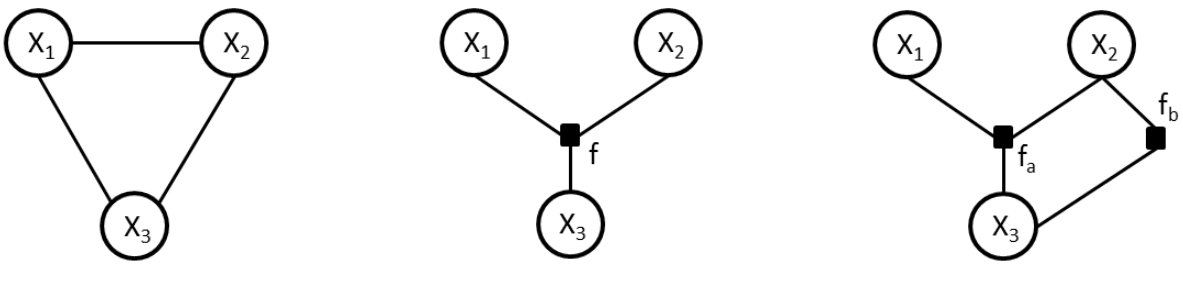
\includegraphics[scale=0.5]{34.png}
\end{center}
\paragraph{Sum-Product Inference} A powerful class of exact inference algorithms. Use factor graph representation to provide a unique algorithm for directed/undirected models. So factor graph are a "unifying language" to represent both models, directed and undirected.\\
Inference is \textbf{feasible for chain and tree structures}. We restructure the graph to obtain a tree-like structure to perform message passing (junction tree algorithm) and then approximated inference (variational, sampling).\\
Even better: we constrain the MRF to obtain tractable classes of undirected models.
\subparagraph{Restricting to Conditional Probabilities} In ML a part of the random variables can be assumed to be always observable (input data).\begin{list}{}{}
	\item $X_k$ are observable inputs in the factor $k$
	\item $Y_k$ are hidden random variables
	\item $f_k(X_k, Y_k)$ is the factor feature function
\end{list}
Instead of $P_\theta(x,y)$ we compute $P_\theta(y\:|\:x)\cdot P_\theta(x)$. Under this assumptio we can directly model the conditional distribution $$P(Y\:|\:X) = \frac{1}{Z(X)}\prod_k \exp\left(\theta_kf_k(X_k,Y_k)\right)$$
We note that $Z$ depends on $X$
$$Z(X) = \sum_y\prod_k\exp\left(\theta_kf_k(X_k,Y_k = y)\right)$$
\subparagraph{Conditional Random Field} CRF are constrained MRF models representing input-conditional distributions.
\begin{center}
	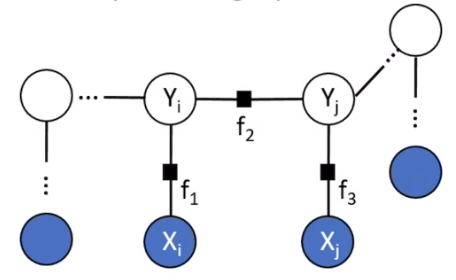
\includegraphics[scale=0.5]{35.png}
\end{center}
\paragraph{Feature Functions} Represent coupling or constraints between random variables, and are often very simple such as linear functions.
\paragraph{Discriminative Learning in Graphical Models} $X$ is always observable input while $Y$ \textbf{can} be unobserved.\\
Let's consider a single $Y$ and multiple $X$s. We can observe the $Y_n$ corresponding to $X_n$ for some $n$, and we can use this information to fit $\theta$ in $P(Y\:|\:X,\theta)$
\paragraph{CRF for Sequences} Undirected and dicriminative equivalent of an HMM.\begin{center}
	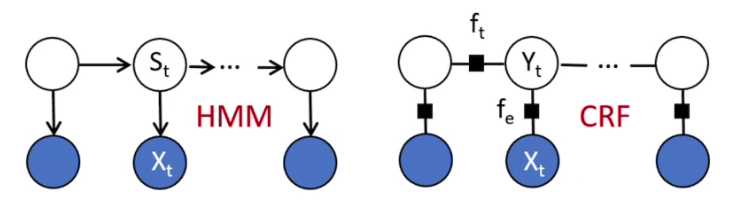
\includegraphics[scale=0.5]{36.png}
\end{center}
Meaning that $f_t(Y_{t-1}, Y_t)$ and it looks like $P(S_t\:|\:S_{t-1})$ of the HMM. $f_e(X_t, Y_t)$ looks like the emission $P(X_t\:|\:S_t)$, but \textbf{I can place as many feature functions $f_t$ I want between the same variables} while I can't place more transition probabilities. The other difference is the main essences.
\paragraph{Generalization of HMM} CRF are much more powerful\begin{center}
	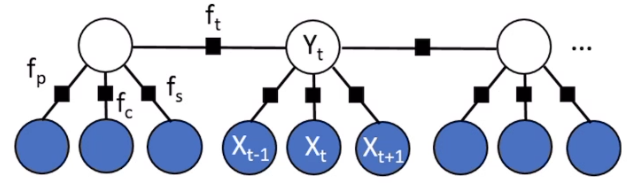
\includegraphics[scale=0.4]{37.png}
\end{center}
Each hidden state may depend on the previous, with $f_t$, but also on the emissions for the previous, current and next symbols. This cannot be easily implemented in HMMs. Kind of time stationality.
$$P(Y\:|\:X,\Theta) = \frac{1}{Z(X)}\prod_t \exp\left(\Theta_pf_p(X_{t-1},Y_t) + \Theta_cf_c(X_t,f_t) + \Theta_sf_s(X_{t+1},Y_t)+\Theta_tf_t(Y_{t-1},Y_t)\right)$$
The cliques to consider are simply $(Y_t, X_{t-1}), (Y_t, X_{t}), (Y_t, X_{t+1}), (Y_t, Y_{t-1})$ for each $t$.\\
We can also model explicitly input influence on transition.
\begin{center}
	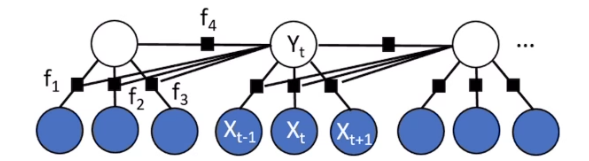
\includegraphics[scale=0.5]{38.png}
\end{center}
The general Linear Conditional Random Fields likelihood is
$$P(Y\:|\:X,\Theta)=\frac{1}{Z(X)}\prod_t\exp\left(\Theta_kf_k(Y_t,Y_{t-1},X_t)\right)$$
Uses indicator variables in $f_k$ definition to include or disregard the influence of specific random variables: e.g. $I_{Y_t=i}, I_{X_t=o}$
\paragraph{Posterior Inference in LCRF} Is there an equivalent of the smoothing problem? Yes: $P(Y_t, Y_{t-1}\:|\:X)$
Solved by exact forward backward inference. Sum-product message passing (alpha-beta recursion) on the LCRF factor graph.
$$P(Y_t,Y_{t-1}\:|\:X)\simeq\alpha_{t-1}(Y_{t-1})\psi_t(Y_t,Y_{t-1},X_t)\beta_t(Y_t)$$
\begin{list}{}{}
	\item \textbf{Clique weighting} $\psi_t(Y_t,Y_{t-1},X_t)=\exp(\Theta_cf_c(X_t,Y_t)+\Theta_tf_t(Y_{t-1},Y_t))$
	\item \textbf{Forward message} $\alpha_t(i) = \sum_j\psi_t(i,j,X_t)\alpha_{t-1}(j)$
	\item \textbf{Backward message} $\beta_t(i) = \sum_i\psi_{t+1}(i,j,X_{t+1})\beta_{t+1}(i)$
\end{list}
Also Viterbi can be used, because we can do Max-Product. The expensive part is the computation of the exponential summation in $Z(X)$. The forward-backward algorithm computes it efficiently as normalization term of $P(Y_t,Y_{t-1}\:|\:X)$. More articulated posteriors interact with $Z(X)$, which is a summation over everything that's not observable, difficult when there's a lot of unobservable variables. Exact inference in CRF other than chain-like is likely to be computationally impractical. We need to approximate: Markov Chain Monte Carlo (sample $y$ rather than estimate $P(y)$) or Variational Belief Propagation (reduce to message passing on trees).
\paragraph{Training LCRF}Maximum (conditional) log-likelihood, for training $$\max_\Theta L(\Theta) = \max_\Theta\sum_{n=1}^n\log P(y^n\:|\:x^n,\Theta)$$
We can substitute the LCRF conditional formulation because $P(y^n\:|\:x^n,\Theta) = \frac{1}{Z(X)}\exp(\sum \Theta_k f_k)$
$$L(\Theta)=\sum_n\sum_t\sum_k \Theta_kf_k(Y_t^n,Y_{t-1}^n,X_t^n)-\sum_n\log Z(X^n)\left(-\sum_k\frac{\Theta_k^2}{2\sigma^2}\right)$$
With the last being a regularization term based on $\|\Theta\|^2$.\\
To get proper marginalization $Z(X^n) = \sum_{y_t,y_{t-1}}\sum_t \exp(\sum_k\Theta_k f_k(y_t,y_{t-1},x^n_t))$\\
With $\frac{\partial L(\Theta)}{\partial \Theta_k}$ we can maximize it because typically $L(\Theta)$ cannot be maximized in closed form.
$$\frac{\partial L(\Theta)}{\partial \Theta_k} = \sum_{n,k}f_k(Y_t^n,Y_{t-1}^n,X_t^n)-\sum_{n,t}\sum_{y,y'}f_k(y,y',X_t^n)P(y,y'\:|\:X^n)-\frac{\Theta_k}{\sigma^2}$$ 
We have sum of expectations: the first term is $E[f_k]$ when $Y$ is not random, with samples drawn from a finite dataset (\textbf{empirical distribution}), and the right term is $E[f_k]$ using the posterior so the expectation of the feature function under the \textbf{model distribution}. $$\frac{\partial L(\Theta)}{\partial \Theta_k} = E[f_k(y,y',x^n_t)] - E_{P(Y\:|\:X,\Theta)}[f_k(y,y',x_t^n)]$$
We need to match those two expectations, meaning that when the gradient is zero these are equal.\\
There's a regularization term $\sum_k\frac{\Theta_k^2}{2\sigma^2}$ on $\|\Theta\|^2$, a posteriori regularization on the gaussian $P(\Theta)$ with $\mu=0$ mean and $\sigma^2I$ variance.\\
In practice, then, $\Theta$ can be learn with stochastic gradient descent or variants.
\paragraph{Applications} Linear CRF have various applications: POS-tagging, semantic role identification, bioinformatics. Feature functions have the form $f_k(X_k,Y_k)=I_{y_k=\hat{y}_k}q(X_c)$, with $f_k$ non-zero only for a specific output configuration $\hat{y}_k$, and then depending only on $X_k$ (the features not shared by the classes). $q(X_c)$ is the observation functions: word begins with capital, ends with -ing\ldots\\
In computer vision they can be used to define bi-dimensioal lattice on images, bg/fg segmentation and to impost constraints.

\subsection{Bayesian Learning and Variational Inference}
Introducing basic concepts of variational learning useful for both generative models and deep learning.
\paragraph{Latent Variables} Unobserved random variables that define a hidden generative process of observed data. They explain complex relation between many observable variables. An example: hidden states in HMM/CRF.\\
Latent variables likelihood $$P(x) = \int_z \prod_{i=1}^N P(x_i\:|\:z)P(z)dz$$ with a graph like $Z \longrightarrow X$ so of nodes $\{Z,X\}$ and a directed arc $(Z,X)$.
\paragraph{Latent Spaces} Spaces where high-dimensional data can be represented. Each of the $M$ samples is made of $N$ features represented with $k<<N$ dimensions.
\begin{center}
	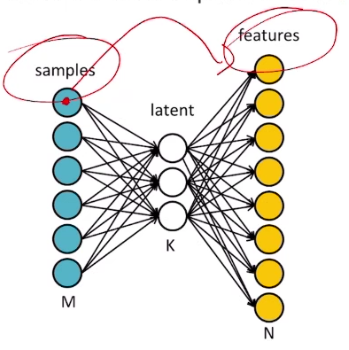
\includegraphics[scale=0.5]{39.png}
\end{center}
The assumption is that latent variables conditional and marginal distribution are more tractable than the joint distribution $P(X)$.
\paragraph{Tractability} Hidden variables can make intractable the posteriors. We need stuff that simplify those posteriors: Bayesian learning introduces priors which introduce integrals in the posteriors computation which are not always analytically or computationally tractable.
\subsubsection{Kullback-Leiber Divergence}
An information thoretic measure of closeness of two distributions $p$ and $q$ $$KL(q\|p) = E_q\left[\log\frac{q(z)}{q(z\:|\:x)}\right] = \langle\log q(z)\rangle_q - \langle\log p(z\:|\:x)\rangle_q$$
Tells how the distribution $q$ differs from $p$. It's a divergence so it is asymmetric, $KL(q\|p) \neq KL(p\|q)$\begin{list}{}{}
	\item if $q$ and $p$ high, then good
	\item if $q$ is high and $p$ is low, the it's unhappy
	\item if $q$ is low we don't care (due to the expectation)
\end{list}
The expectation $E_q$ means taking all possible assignments $z$ weighted according to the probability $q(z)$.
\paragraph{Jensen Inequality} Property of linear operators on convex/concave functions $$\lambda f(x) + (1-\lambda)f(x)\geq f(\lambda x + (1-\lambda)x)$$
The curve is longer than the line connecting the two points. With concave we have $\leq$. Applied to probability $$f(E[X])\geq E[f(X)]$$
$$\log(E[X])\geq E[\log(X)]$$
The log-likelihood for a model with a single hidden variable $Z$ and parameters $\theta$ with a single sample assumed for simplicity is the following
$$\log P(x\:|\:\Theta) = \log\int_zP(x,z\:|\:\Theta)dz = \log\int_z\frac{Q(z\:|\:\phi)}{Q(z\:|\:\phi)}P(x,z\:|\:\Theta)dz$$
$Q$ is a distribution, used over $z$ with parameters $\phi$ and $Q(z\:|\:\phi)\neq 0$. That is the definition of expectation, we have $\int_zQ(z\:|\:\phi)\cdot \frac{1}{Q(z\:|\:\phi)}P(x,z\:|\:\Theta)$ which is $\sum_z q\cdot g(z)$. Using Jensen we have $$\log P(x\:|\:\Theta)= \log E_Q\left[\frac{P(x,z)}{Q(z)}\right] \geq E_Q\left[\log \frac{P(x,z)}{Q(z)}\right]= E_Q[\log P(x,z)] - E_Q[\log Q(z)] = L(x,\Theta,\phi)$$
So we are lower bounding $\log P(x\:|\:\Theta)$ with the expected joint distribution minus the entropy. So we have a lower bound on something I want to maximize, so we can maximize the lower bound. Maximizing this term entails that we're supported by the data (using the expectation of joint distribution $E_Q[\log P(x,z)]$).\\
How good is this lower bound? Meaning $\log P(x\:|\:\Theta) - L(x,\Theta,\phi) = ?$ We introduce $Q(z)$ by marginalization $$\int_z Q(z)\log P(x) - \int_z Q(z)\log\frac{P(x,z)}{Q(z)} = \int_z Q(z)\log\frac{P(x)Q(z)}{P(x,z)}=E_Q\left[\log \frac{Q(z)}{P(z\:|\:x)}\right] = KL\left(Q(z\:|\:\phi)\|P(z\:|\:x,\Theta)\right)$$
Because $\frac{P(x)}{P(x,z)} = \frac{1}{P(z\:|\:x)}$. So it's an optimization problem of finding $\Theta$ and $\phi$ that maximize $L(x,\Theta,\phi)$ reduced to a minimization problem with KL.\\
We can assume the existence of a probability $Q(z\:|\:\phi)$ which allows to bound the likelihood $P(x\:|\:\Theta)$ from below using $L(x,\Theta,\phi)$.\\
$L(x,\Theta,\phi)$ is called \textbf{variational bound} or \textbf{ELBO} (evidence lower bound). The optimal bound is obtained from $KL\left(Q(z\:|\:\phi)\|P(z\:|\:x,\Theta)\right) = 0$ choosing $Q(z\:|\:\phi)=P(z\:|\:x,\Theta)$. So the problem now becomes maximizing ELBO $$\max_{\Theta,\phi}\sum_{n=1}^N L(x_n,\Theta,\phi)$$ where $\Theta$ are the model parameters and $\phi$ is used in $Q(z\:|\:\phi)$.\\
If $P(z\:|\:x,\Theta)$ is tractable then we use it s $Q(z\:|\:\phi)$ (optimal ELBO). Otherwise we choose $Q(z\:|\:\phi)$ as a tractable family of distributions: find $\phi$ that minimize $KL(Q(z\:|\:\phi)\|P(z\:|\:x,\Theta))$ or find $\phi$ that maximize $L(\:,\phi)$.
\paragraph{Example} Bag of Words representations are classical examples of multinomial data. A BOW dataset $X$ is the $N\times M$ document matrix, with $N$ number of vocabulary items $w_j$ and $M$ is the number of documents $d_i$ and $x_{ij} = n(w_j,d_i)$ the number of occurrences of $w_j$ in $d_i$.\\
Often $M$ is very very large ($\simeq 30$k elements). So we want a smaller representation. Mixture of topics: a topic identifies a pattern in the co-occurrence of multinomial items $w_j$ within the documents. Mixture, so we associate an interpretation (topic) to each item in a document, whose interpretation is then a mixture of the items' topics. We use Latent Variables.
\paragraph{Latent Dirichlet Allocation} LDA models a document as a mixture of topics $z$. We assign one topic $z$ to each item $w$ with probability $P(w\:|\:z,\beta)$ and pick a topic for the whole document with probability $P(z\:|\:\Theta)$
\begin{center}
	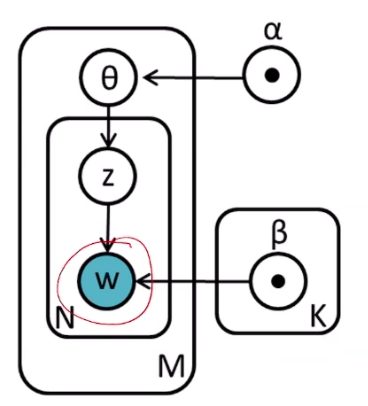
\includegraphics[scale=0.5]{40.png}
\end{center}
Each document has its personal topic proportion $\Theta$ sampled from a distribution. $\Theta$ defines a multinomial distribution, but it is a random variable as well. $\alpha$ is the prior.
\paragraph{Dirichlet distribution} Conjugate prior to multinomial distribution.\\
If the likelihood is multinomial with a Dirichlet prior, then posterior is Dirichlet.
$$P(\Theta\:|\:\alpha) = \frac{\Gamma(\sum_{k=1}^K \alpha_k)}{\prod_{k=1}^K\Gamma(\alpha_k)}\prod_{k=1}^K\Theta_k^{\alpha_k-1}$$
$\Gamma$ is the generalization of the factorial. With a big $\alpha$ we make the topics almost equiprobable, while with lower $\alpha$ we get substatially different proportions (less and less topics active). So big $\alpha$ means that every document can express each topic, while low $\alpha$ is almost deterministic. Usually, $\alpha = 1$ or similar but smaller.\\\\
LDA finds a set of $K$ projection functions on the $K$-dimensional topic simplex.\begin{center}
	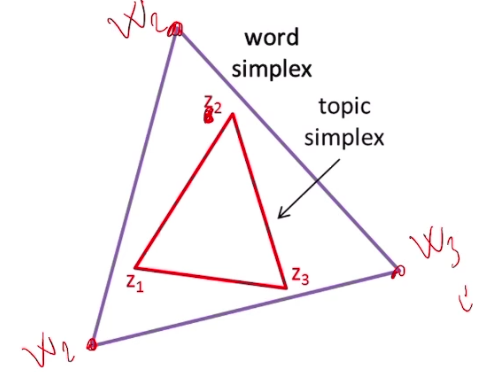
\includegraphics[scale=0.5]{41.png}
\end{center}
\paragraph{LDA Generative Process} For each of the $M$ documents, we choose $\Theta$ with Dirichlet($\alpha$) and for each of the $N$ items, we choose a topic $z$ with Multinomial($\Theta$) and pick an item $w_j$ with multinomial probability $P(w_j\:|\:z,\beta)$.\\
We get a multinomial topic-item parameter matrix $[\beta]_{k\times V}$
$$\beta_{kj}=P(w_j=1\:|\:z_k=1)\hbox{ or } P(w_j=1\:|\:z=k)$$
$$P(\Theta, z, w\:|\:\alpha,\beta) = P(\Theta\:|\:\alpha)\prod_{j=1}^NP(z_j\:|\:\Theta)P(w_j\:|\:z_j,\beta)$$
It's a completed likelihood with the conditional independence assumption.
\subparagraph{Learning} Marginal distribution of a document $d =$ w
$$P(\hbox{w}\:|\:\alpha,\beta) = \int \sum_z P(\Theta,z,w\:|\:\alpha,\beta)d\Theta=\int P(\Theta\:|\:\alpha)\prod_{j=1}^N\sum_{z_j=1}^kP(z_j\:|\:\Theta)P(w_j\:|\:z_j,\beta)d\Theta$$
given w$_1$,\ldots,w$_M$ find $\alpha,\beta$ that maximize.\\
Key problem is inferring latent variables posterior:
$$P(\Theta, \hbox{z}\:|\:\hbox{w},\alpha,\beta) = \frac{P(\Theta, \hbox{z}, \hbox{w}\:|\:\alpha,\beta)}{P(\hbox{w}\:|\:\alpha,\beta)}$$
but the denominator is intractable because of couplings between $\beta$ and $\Theta$ under exponenziation in the summation over topics. So we don't use the posterior, we pick a function $Q$ that helps in solving the problem (variational inference).
\paragraph{Variational Inference} We write $Q(z\:|\:\phi)$ function that is sufficiently similar to the posterior but tractable. It should be such that $\beta$ and $\Theta$ are no longer coupled, fitting $\phi$ so that is close to the posterior according to KL.\\
Fast convergence but it's an approximation.\\
The key idea is to assume that $Q(z\:|\:\phi)$ is tractable: \textbf{mean-field assumption}.
$$Q(z\:|\:\phi) = Q(z_1,\ldots,z_K\:|\:\phi)=\prod_{k=1}^K Q(z_k\:|\:\phi_k)$$
Can be generalized by factorizing on groups of latent variables. Does not contain the true posterior because hidden variables are dependent.\\
We optimize ELNO using $Q(z\:|\:\phi)$ using the factorized distribution. Simple \textbf{coordinate ascent inference}: iteratively optimize each variational distribution holding the others fixed, so when learning we use the model on the right, breakdown of the independence.\begin{center}
	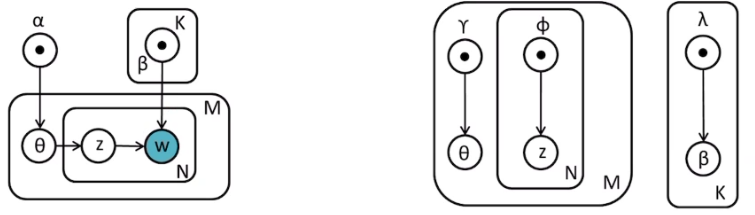
\includegraphics[scale=0.5]{42.png}\\
	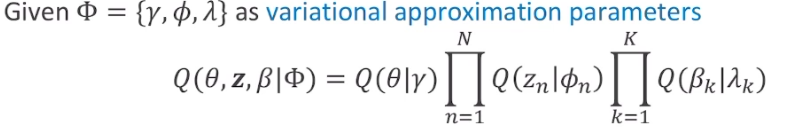
\includegraphics[scale=0.5]{43.png}
\end{center}
\paragraph{Variational Expectation-Maximization} Find the $\Phi, \Psi$ that maximize the ELBO
$$L(w,\Phi,\Psi) = E_Q[\log P(\Theta,z,w\:|\:\Psi)] - E_Q[\log Q(\Theta,z,\Psi\:|\:\Phi)]$$
by alternate maximization:
\begin{list}{}{}
	\item Fix $\Psi$ and update variational parameters $\Psi^*$ (\textbf{E-Step})
	\item Fix $\Phi = \Phi^*$ and update the model parameters $\Psi^*$ (\textbf{M-Step})
	\item Repeat until little improvement on the likelihood
\end{list}
Unlike EM, variational EM has no guarantee to reach a local maximizer of $L$.
\subsection{Boltzmann Machines}
Examples of Markov Random Fields:
\begin{list}{}{}
	\item Visible random variables $v\in\{0,1\}$
	\item Latent random variables $h\in\{0,1\}$
	\item $s = [vh]$ (concatenation)
\end{list}
\begin{center}
	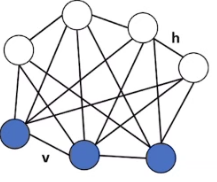
\includegraphics[scale=0.5]{46.png}
\end{center}
Linear energy function $$E(s) = -\frac{1}{2}\sum_{ij}M_{ij}s_is_j - \sum_jb_js_j = -\frac{1}{2}s^TMs - b^Ts$$
with symmetric and no self-recurrent connectivity. Model parameters $\Theta = \{M, b\}$ encode the interactions between the variables (observable and not).\\
\textbf{Boltzmann machines are a type of Recurrent Neural Networks}. They can be interpreted as stochastic neural network: the state of a unit at a given timestep is sampled from a given probability distribution and the network learns a probability distribution $P(V)$ from the training patterns. The network includes both visible $v$ and hidden $h$ units, and the activity is a sample from posterior probability given the inputs (visible data).
\paragraph{Stochastic Binary Neurons} Binary output $s_j$ at any time $t$. Typically discrete time model with time into small $\Delta t$ intervals. At each time interval $t+1 = t+\Delta t$ the neuron can emit a spike with probability $p_j^{(t)}$ $$s_j^{(t)} = \left\{\begin{array}{c l}
1&\hbox{with probability }p_j^{(t)}\\
0&\hbox{with probability }1-p_j^{(t)}
\end{array}\right.$$
The key is in the definition of the spiking probability (local potential $x_j$ $$p_j^{(t)} \simeq \sigma(x_j^{(t)})$$
The Boltzmann machine has $N$ neurons with binary activations $s_j$, a weight matrix $M = [M_{ij}]_{i,j} \in \{1,\ldots,N\}$ and a bias vector $b = [b_j]_j\in\{1,\ldots,N\}$\\
Local neuron potential $x_j$ is the usual $$x_j^{(t+1)} = \sum_{i=1}^N M_{ij}s_j^{(t)} +b_j$$
This assuming full connectivity with weight $0$ if you want to ignore a neuron in the potential. A chosen neurpon fire with spiking probability which is a sigmoid $$p_j^{(t+1)} = P(s_j^{(t+1)} = 1\:|\:s^{(t)}) = \sigma(x_j^{(t+1)}) = \frac{1}{1+e^{-x_j^{(t+1)}}}$$
Clearly has Markovian dynamics, $P(s^{t+1}\:|\:s^t)$\\\\
How does the model state (activation of all neurons) evolve in time?
\paragraph{Parallel Dynamics} Assuming we can compute each activation in parallel every $\Delta t$, updating each random variable in parallel. $$P(s^{t+1}\:|\:s^t) = \prod_{j=1}^N P(s_j^{t+1}\:|\:s^t) = T(s_j^{t+1}\:|\:s^t)$$
Yielding a Markov process for state update
$$P(s^{t+1} = s') = \sum_s T(s'\:|\:s)P(s^t = s)$$
\paragraph{Glauber Dynamics} One neuron at random is chosen for update at each step. No fixed-point guarantees for $s$, but it has a stationary distribution for the network at equilibrium state when its connectivity is symmetric.
\subparagraph{Boltzmann-Gibbs Distribution} Undirected connectivity enforces detailed balance condition $$P(s)T(s'\:|\:s) = P(s')T(s\:|\:s')$$
Ensures reversible transitions guaranteeing existence of equilibrium distribution (Boltzmann-Gibbs) $$P_\infty(s) = \frac{e^{-E(s)}}{Z}$$
where $E(s)$ is the energy function and $Z = \sum_se^{-E(s)}$ is the partition function.
\paragraph{Learning} Boltzmann machines can be trained so that the equilibrium distribution tends towards any arbitrary distribution across binary vectors given samples from that distribution. Basically, you can represent any distribution of binary variables.\\
Couple of simplifications:
\begin{list}{}{}
	\item bias $b$ is just another row in the weight matrix $M$
	\item consider only visible random variables, meaning $s = v$
\end{list}
We use probabilistic learning techniques to fit the parameters, i.e. maximizing the log-likelihood $$L(M)=\frac{1}{L}\sum_{l=1}^L \log P(v_l\:|\:M)$$
given the $P$ visible training patterns $v_l$, the set of all the visible units (so it's a joint distribution $v_{l1},\ldots,v_{ln}$. We need a way to write the likelihood $P(v_l\:|\:M)$, and we can use the Boltzmann-Gibbs. So we can optimize it solving a maximum likelihood problem.
$$\log P(v_l\:|\:M) = \log \frac{e^{-E(v)}}{Z} = -E(v) - \log Z$$
$$\frac{\partial L}{\partial M_{ij}} \Rightarrow \frac{\partial (-E(v) - \log Z)}{\partial M_{ij}}\Leftrightarrow$$
Given that $E(v) = -\frac{1}{2}v^TM^Tv = -\sum_{ij} M_{ij} v_1v_j$ we get that every $M_{ij}$ will be constant except for the $M_{ij}$ we are differentiating leaving with $v_iv_j$. As for $\log Z$, differentiating the potential function leaves us with $\sum_v P(v\:|\:M)v_iv_j$ from $\partial\log\partial\exp\cdot\partial E$
$$\Leftrightarrow v_iv_j - \sum_v P(v\:|\:M)v_iv_j = 0$$
The second term is $\sum_v P(v\:|\:M)v_iv_j = E_{v_iv_j\in P(v\:|\:M)}[v_iv_j] = \langle v_iv_j\rangle_M$ the expectation of the coactivation of two units $v_i,v_j$ when the values of those two units are taken from $P(v\:|\:M)$ the distribution learned by the model $M$.\\
So for a single $l$:
$$v_i^lv_j^l - \langle v_iv_j\rangle_M$$
not introducing $l$ in the second term because it's marginalized, all the possible values in all possible configurations, it's an expectation and the data is already included in the formulation.\\
So $\forall\:v^l\in L$ $$\frac{\partial L}{\partial M_{ij}} = \frac{1}{L}\sum_{l=1}^L (v_i^lv_j^l)-\langle v_iv_j\rangle_M=$$
We have the clamped expectation under the empirical distribution $\frac{1}{L}\sum_{l=1}^L (v_i^lv_j^l) = E_{v_i^lv_j^l\in L}[v_i^lv_j^l] = \langle v_iv_j\rangle_c$
$$=\langle v_iv_j\rangle_c - \langle v_iv_j\rangle_M = \Delta M_{ij}$$
So we're focusing on the neurons $i, j$ and the link between them $M_{ij}$, and we increase the connection when both are 1 so when $\langle v_iv_j\rangle_c$ is larger, so Hebbian learning. The second term $\langle v_iv_j\rangle_M$, if they are in disagreement then they are flipped then it's zero, if instead they are coactive (both on or off) then it's close to $-1$. It's anti-Hebbian, has the purpose of nearing the expectation of the model towards the reality.\\
When $\langle v_iv_j\rangle_c - \langle v_iv_j\rangle_M = 0-1$, we get that the model thinks that they are correlated while the are different, so the model stop believing that they are correlated.\\\\
With hidden variables doesn't change much. We have $s=[hv]$
The wake hebbian term $\sum_h s_is_jP(h\:|\:v)$ and the dream anti-hebbian term $\sum_ss_is_jP(s)$
$$\frac{\partial P(v\:|\:M)}{\partial M_{ij}} = \sum_h s_is_jP(h\:|\:v) - \sum_ss_is_jP(s) = \langle s_is_j\rangle_c - \langle s_is_j\rangle_M = \Delta M_{ij}$$
Again intractable. So we restrict.
\paragraph{Restricted Boltzmann Machines} RBM are special Boltzman machines: bipartite graphs and connections only between hidden and visible units, not with "themselves".
\begin{center}
	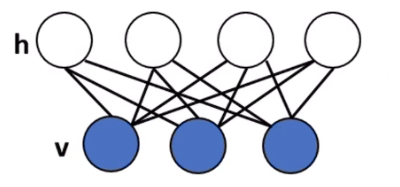
\includegraphics[scale=0.5]{47.png}
\end{center}
This becomes tractable because we can compute the activation of each hidden in parallel and then compute the visible. The energy function is a specialization that higlights the bipartition in hidden and visible units $$E(v,h) = -v^TMh - b^Tv - c^Th$$
Hidden units are conditionally independent given visible units and viceverse
$$P(h_j\:|\:v)=\sigma\left(\sum_i M_{ij}v_i+c_j\right)$$
$$P(c_i\:|\:v)=\sigma\left(\sum_j M_{ij}h_j+b_i\right)$$
Training is again based on the likelihood maximization $$\frac{\partial L}{\partial M_{ij}} =\langle v_ih_j\rangle_c -\langle v_jh_j\rangle = \Delta M_{ij}$$
Again, we have data $-$ model which are both expectations that need to be estimated. The first has the sum on just $h$, the second is a full summation over both $v$ and $h$.\\
With a Gibbs sampling approach, for the wake/data term\begin{list}{}{}
	\item clamp data on $v$
	\item sample $v_i,h_j$ for all pairs of connected units
	\item Repeat for all elements of dataset
\end{list}
as to stay as much as possible to the empirical data, and for the model/dream term\begin{list}{}{}
	\item 
\end{list}
computing a correlation between ideally $v^\infty,h^\infty$, but of course can't wait until the infinity sample and we cut at some sample $k$ so $v^k,h^k$.
\begin{center}
	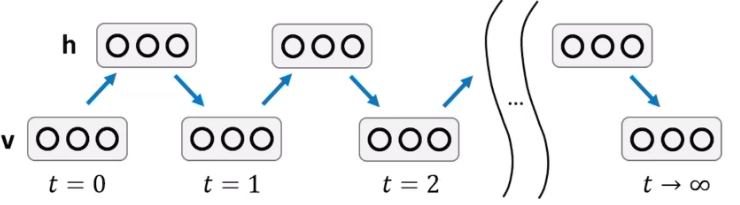
\includegraphics[scale=0.5]{48.png}
\end{center}
We start with a training vector on the visible units, alternating between updating all the hidden units in parallel and updating all the visibile units in parallel
$$\frac{\partial L}{\partial M_{ij}} = \langle v_ih_i\rangle_0 - \langle v_jh_j\rangle_\infty = \hbox{data} - \hbox{model}$$
\paragraph{Contrastive-Divergence Learning} Because Gibbs sampling converges really slowly: clamp a training vector $v^l$ on visible units. CD-1.
\begin{center}
	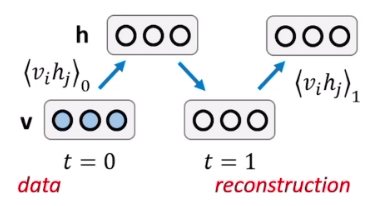
\includegraphics[scale=0.5]{49.png}
\end{center}
Clamping a training vector $v^l$ on visible units, update all hidden units in parallel, update all the visible units in parallel to get a \textbf{reconstruction} and update the hidden units again.
$$\begin{array}{c c c}
\langle v_ih_j\rangle_0&-&\langle v_ih_j\rangle_1\\
\hbox{data}& &\hbox{reconstruction}
\end{array}$$
Learns a very crude approximation of the gradient of log-likelihood, not even following it closely. Why use it? Because in practice it works well.

\subsection{Wrap Up}
We've seen three families of models\begin{list}{}{}
	\item \textbf{Bayesian Networks}: unsupervised data understanding, interpretability but weak on supervised performance. Directed.
	\item \textbf{Markov Random Fields}: undirected version of BN, powerful when knowledge and constraints can be expressed with dictionaries. CRF: supervised way to be generative.\\
	But computationally heavy.
	\item \textbf{Dynamic Models}: topology unfolds on data structure, structured data processing but complex causal relationships.
\end{list}
\paragraph{Tractability} Generative models to be used when:
\begin{list}{}{}
	\item Need interpretability
	\item Need to incorporate prior knowledge
	\item Unsupervised learning or learning with partially observable supervision
	\item Need reusable/portable knowledge
\end{list}
To be avoided when:
\begin{list}{}{}
	\item Having tight computational constraints
	\item Dealing with raw, noisy, low-level data
\end{list}
Variational inference and sampling are efficient ways to learn approximations to intractable distribution. Neural networks can be used as variational functions or to implement sampling processes.
\section{Sampling Methods} 
\paragraph{Probability Recap}
\paragraph{Sampling} Drawing a set of realisations $X = \{x_1,\ldots,x_L\}$ of a random variable $x$ with a distribution $p(x)$. The set contains $L$ samples.\\
If we have a sampling set we can use it to approximate $p(x)$ $$p(x)\simeq \frac{1}{L}\sum_{l=1}^L I[X_l = i]$$ with $I[c] = 1 \Leftrightarrow c$ is true.\\
We can also approximate the expectation of a function $f$ $$E_{p(x)}[f(x)]\simeq \frac{1}{L}\sum_{l=1}^L f(x_l)$$
We need sampling when $p(x)$ is intractable. For example, in Bayesian models the parameters are random variables but the posteriors are often intractable so we can use sampling to obtain the model parameters.
\paragraph{Sampling Procedure as Distributions} A sampler $S$ is a procedure that generates a sample set $X$ from a generic distribution $p(x)$. Since $X$ contains realizations of random variables, also $X$ has a probability distribution. We denote with $\hat{p}_S(X)$ the probability to obtain the sample set $X$ from the sampler $S$.\\
A \textbf{sampler} and its properties \textbf{are fully defined by its distribution} $\hat{p}_S(X)$. In general
$$\hat{p}(X) \neq p(x)$$
\begin{list}{}{}
	\item $p(x)$ is the distribution we would like to sample from, usually intractable
	\item $\hat{p}(X)$ is the distribution over the samples set and defined by the sampling procedure
\end{list}
Let us consider the sampling approximation of the expectation
$$E_{p(x)}[f(x)]\simeq \frac{1}{L}\sum_{l=1}^L f(x_l) = \hat{f}_X$$
Since $\hat{f}_X$ estimates a value, we could ask:
\begin{list}{}{}
	\item Is $\hat{f}_X$ an unbiased estimator?
	\item How much is the variance of the approximation?
\end{list}
An unbiased estimator $\hat{\Theta}$ of the unknown $\Theta \Rightarrow$ the approximation is exact on average. Meaning: let $\hat{p}(X)$ the distribution over all possible realizations of the sampling set $X$, then $\hat{f}_X$ is unbiased estimator if $$E_{\hat{p}(X)}[\hat{f}_X] = E_{p(x)}[f(x)]$$
This is true provided that $\hat{p}(x_l) = p(x_l)$\\
A sampler with this property is called \textbf{valid} because it draws samples from the desired distribution.\\\\
The variance of $\hat{f}(X)$ tells us how much we can rely on the approximation computed using the sampling set $X$. Let $$\Delta\hat{f}_X = \hat{f}_X - E_{\hat{p}(X)}[\hat{f}_X]$$ then the variance of $\hat{f}(X)$ is given by $$E_{\hat{p}_X}[(\Delta\hat{f}_X)^2]$$
we would like low variance meaning that $\hat{f}(X)$ is quite always close to the average, i.e. to $E_{p(X)}[f(X)]$.\\\\
So if the sampler has same marginals and draws sample independently we obtain $$E_{\hat{p}_X}[(\Delta \hat{f}_X)^2] = \frac{1}{L}\hbox{Var}_{p(x)}[f(x)]$$
The variance reduces linearly with respect to the number of samples provided that $\hbox{Var}_{p(x)}[f(x)]$ is finite.\\\\
We've shown that we need sampling to approximate expectations and to do inference in Bayesian models. Propertis of the sampling procedure depends on $\hat{p}(X)$: valid sampler and low approximation variance.
\subsection{Univariate Sampling}
Easy: random number generator $R$ which produces a value uniformly at random in $[0,1]$ and $p(x)$. We use $p(x)$ to divide $[0,1]$ in bins and sample accordingly.
\subsection{Multivariate Sampling}
In the multivariate case $p(x)$ represents a joint distribution over a set of discrete variables $\{s_1,\ldots,s_n\}$ each with $C$ states. Hence each sample $x_i\in X$ contains $n$ values.\\
We build a univariate distribution $p(S)$ where $S$ is a discrete variables with $C^n$ states (all possible combinations) and we can sample from $p(S)$ using the univariate schema.
\begin{center}
	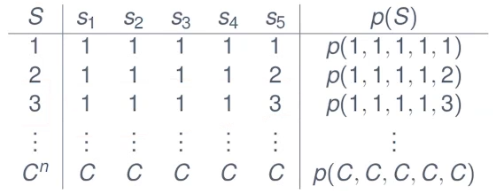
\includegraphics[scale=0.5]{44.png}
\end{center}
The problem is the number of possible states $C^n$, so computationally unfeasible.\\
Using the chain rule we can rewrite the joint distribution as a chain of conditional distributions. Then we sample in order:
\begin{list}{}{}
	\item $\hat{s}_1 \simeq p(s_1)$
	\item $\hat{s}_2 \simeq p(s_2\:|\:\hat{s}_1)$
	\item \ldots
	\item $\hat{s}_n \simeq p(s_n\:|\:\hat{s}_1,\ldots,\hat{s}_{n-1})$
\end{list}
Each is univariate, so easy, but unfortunately computing the distribution $p(s_i\:|\:s_{j<i})$ often requires summation over an exponential number of states.\\
This approach is called \textbf{Ancestral Sampling}. There are cases where it cannot be used.
\subparagraph{Example} We can apply directly if a distribution $p(s_1,\ldots,s_n)$ is already presented as a belief network:
\begin{center}
	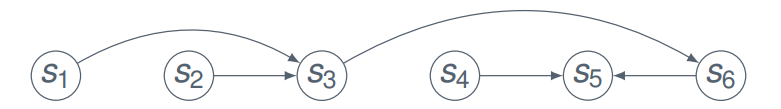
\includegraphics[scale=0.5]{67.png}
\end{center}
The BN ancestral order tells us the sampling order
$$\{s_1,s_2,s_4\}\prec\{s_3\}\prec\{s_6\}\prec\{s_5\}$$\begin{list}{}{}
	\item Sample $\hat{s}_1\simeq p(s_1)$
	\item Sample $\hat{s}_4\simeq p(s_4)$
	\item Sample $\hat{s}_2\simeq p(s_2)$
	\item Sample $\hat{s}_3\simeq p(s_3)$
	\item Sample $\hat{s}_6\simeq p(s_6)$
	\item Sample $\hat{s}_5\simeq p(s_5)$
\end{list}
We obtain a single sample $x^l = \hat{s}_1,\hat{s}_2,\hat{s}_3,\hat{s}_4,\hat{s}_5,\hat{s}_6$.\\\\
Suppose a subset $s_\epsilon$ of variables that are visible, with $s=s_\epsilon\cup s_{\setminus\epsilon}$ we want to sample from $$P(s_{\setminus\epsilon}\:|\:s_\epsilon) = \frac{p(s_{\setminus\epsilon}, s_\epsilon)}{p(s_\epsilon)}$$
Can we still use Ancestral Sampling?\begin{list}{}{}
	\item Clamping variables changes the structure of the bayesian network, and computing the new structure is as complex as running exact inference.
	\item We could run AS on the original structure and discarding any samples which do not match the evidence.
\end{list}
Sampling under evidence is very important, in probabilistic models the inference is based on the posterior which is exactly that. So we need an efficient method of sampling under evidence.
\paragraph{Gibbs Sampling Procedure}
The idea is to start from a sample $x^1=\{s_1^1,\ldots,s_n^1\}$ and \textbf{update only one variable at a time}. Dealing with evidence is easy, we just do not select the visible variables.\\
During the $(l+1)$th iteration:
\begin{list}{}{}
	\item Select a variable $s_j$
	\item we sample the new value according to $$s_j^{l+1}\simeq p(s_j\:|\:s_{\setminus j}) = \frac{1}{Z}p(s_j\:|\:\hbox{Parents}(s_j))\prod_{k\in\hbox{Children}(s_j)} P(s_k\:|\:\hbox{Parents}(s_k)) $$
\end{list}
Which depends only on the Markov blanket of $s_j$ and $s_{\setminus j}$ is clamped to$ \{s_1^l,\ldots,s_{j-1}^l,s_{j+1}^l,\ldots,s_n^l\}$
\begin{center}
	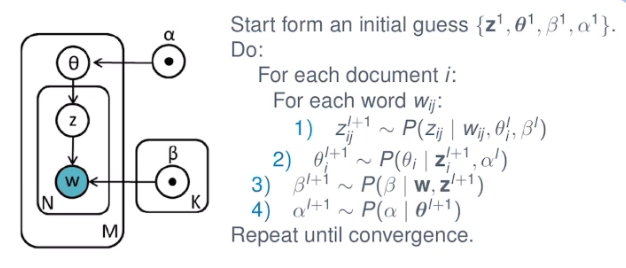
\includegraphics[scale=0.5]{45.png}
\end{center}
\subparagraph{$\hat{p}(X)$ of Gibbs sampling} Considering a set of variables $X=\{x^1,\ldots,x^L\}$ obtained with a Gibbs sampler: each sample $x^{l+1}$ is obtained from the previous sample $x^l$. We can define a probability $q(x^{l+1}\:|\:x^l)$, the probability to obtain $x^{l+1}$ given $x^l$:
$$q(x^{l+1}\:|\:x^l) = \sum_{j=1}^NP(\hbox{Variable }j\hbox{ is selected})P(\hbox{New value }s_j^l\hbox{ given }x^l)$$
With $P(\hbox{New value }s_j^l\hbox{ given }x^l)$ from equation 4 and $P(\hbox{Variable }j\hbox{ is selected})$ up to you.\\
With this we can compute $\hat{p}(X)$ $$\hat{p}(X)=\prod_{l=1}^L q(x^{l+1}\:|\:x^l)$$
\paragraph{Markov Chain Monte Carlo Sampling Framework} Gibbs sampling is a specialization of the Markov Chain Monte Carlo sampling framework. The idea is to build a Markov Chain whose stationary distribution is $p(x)$.\\
Let $q(x^{l+1}\:|\:x^l)$ be the Markov Chain state-transition distribution, if the Markov Chain is\begin{list}{}{}
	\item \textbf{Irreducible}, meaning it's possible to reach any state from anywhere
	\item \textbf{Aperiodic}, meaning at each time-step we can be anywhere
\end{list}
then it has a unique stationary distribution. So we define $q(x^{l+1}\:|\:x^l)$ such that the Markov Chain converges to $p(x)$.
\section{Convolutional Neural Networks}
\paragraph{Deep Learning} Effectively is learning the representation of data.
\paragraph{CNNs} The principle is complex neurons that take the outputs of simple neurons and assemble it into more complex structures.
\begin{multicols}{2}
For sequences:
\begin{center}
	\includegraphics[scale=0.5]{66.png}
\end{center}
Apply a bank of 16 convolution kernels to sequences (window of 15 elements) trained by backpropagation with parameter sharing.
\columnbreak

For images:
\begin{center}
	\includegraphics[scale=0.35]{50.png}
\end{center}
\end{multicols}

\paragraph{Dense Vector Multiplication} E.g. take the 32x32 image and reshape into a vector of 3072. Input-sized weight vector for each hidden neuron $W$ of e.g. 100 neurons: 100$\times$3072 weights, a huge amount of parameters. That's why we want convolutional filters.
\begin{center}
	\includegraphics[scale=0.5]{51.png}
\end{center}
A set of weights that are applied to a 5$\times$5 region of the image. It's a \textbf{kernel} that outputs into the \textbf{feature map}. No longer a 1:1 correspondence between a pixel and a parameter.
\begin{center}
	\includegraphics[scale=0.5]{52.png}
\end{center}
\begin{center}
	\includegraphics[scale=0.5]{53.png}
\end{center}
With a number of slices equal to the number of image channels. Basically a filter per channel color, but they are convolved together still giving a $28\times28$ feature map even with 3 color channels for example. The \textbf{convolution map stays bidimensional}.
\paragraph{Stride} Basic convolution slides the filter on the image one pixel at the time (stride = 1). The slide value is an hyperparameter. The stride reduces the number of multiplication, sumbsampling the image. With a stride of 2 for example we would end up with a $14\times14$ map.
\paragraph{Activation Map Size} What is the size of the image after applying a filter with a given stride $S$ and size $K\times K$, on a image $W\times H$?\\
For example, a $3\times 3$ filter with stride $2$, $K=3, S=2$ on a $7\times 7$ image: output image is $3\times 3$.
$$W'=\frac{W-K}{S}+1$$
$$H'=\frac{H-K}{S}+1$$
\paragraph{Zero Padding} Add columns and rows of zeros to the border of image to handle border pixels, padding of $P$ rows/columns.
$$W'=\frac{W-K+2P}{S}+1$$
Zero padding is also used to retain the original size of the image
$$P=\frac{K-1}{2}$$
\paragraph{Feature Map Transformation} Convolution is a linear operator, applying an element-wise nonlinearity we obtain a transformed feature map.
$$\max(0, w^Tx_{ij} + b)$$
The above is ReLU, used because of the simplicity of computing the gradient.
\paragraph{Pooling} Operates on the feature map to make the representation: smaller (subsampling) and robust to some transformations.\\
Very simple: \begin{center}
	\includegraphics[scale=0.5]{54.png}
\end{center}
Max pooling is the one used more frequently, but there's more: average pooling, L2-norm pooling, even random pooling.\\
It's uncommon to use zero padding with pooling.
$$W' = \frac{W-K}{S} + 1$$
\paragraph{Convolutional Architecture}
\begin{center}
	\includegraphics[scale=0.5]{55.png}
\end{center}
Usually use a certain number of convolutional layers ending in a small final image feeded into some fully connected layers.
\paragraph{Filter Banks}
\begin{center}
	\includegraphics[scale=0.5]{56.png}
\end{center}
The number of parameters in this model is $K\times K\times D_I\times D_K$ because pooling is non parametric and feature maps have no parameters, so the parameters are just in the filters.
\paragraph{CNNs as Sparse Neural Networks}
Let's use a 1D input sequence to ease graphics.
\begin{center}
	\includegraphics[scale=0.5]{57.png}
\end{center}
Convolution amounts to sparse connectivity (reduce parameters) with parameter sharing (enforces variance).\\
$s_i$ is a convolutional neuron with a kernel size $3\times1$
\subparagraph{Strided Convolution} A neuron after every stride, making connectivity sparser.
\begin{center}
	\includegraphics[scale=0.5]{58.png}
\end{center}
\subparagraph{Pooling} Just another neuron.
\begin{center}
	\includegraphics[scale=0.5]{59.png}
\end{center}
\subparagraph{Cross-Channel Pooling and Spatial Invariance}
\begin{center}
	\includegraphics[scale=0.5]{60.png}
\end{center}
\subparagraph{Hierarchical Feature Organization}
\begin{center}
	\includegraphics[scale=0.5]{61.png}
\end{center}
\paragraph{CNN Training}
Training by variants of the standard backpropagation that account for the fact that connections share weights (convolution parameters).
\begin{multicols}{2}
\begin{center}
	\includegraphics[scale=0.5]{62.png}
\end{center}
The gradient $\Delta w_i$ is obtained by summing the contributions from all the connections sharing that weight.\\
We can write convolution as dense multiplication with shared weights.
\end{multicols}
\paragraph{Deconvolution}
\begin{center}
	\includegraphics[scale=0.5]{63.png}
\end{center}
We can obtain the transposed convolution using the same logic of the forward convolution. If you had no padding in the forward convolution you need to use much padding when doing the transposed convolution.
\paragraph{ReLU} ReLU helps counteract gradient vanish: sigmoid first derivative vanishes as we increase or decrease $z$, ReLU first derivative is 1 when unit is active and 0 otherwise. ReLU second derivative is 0 (no second order effects).\\
Easy to compute and favors sparsity.
\paragraph{VGGNet} Standardized convolutional layer:
\begin{list}{}{}
	\item 3$\times$3 convolutions of stride 2
	\item 2$\times$2 convolutions of stride 2
	\item 16 convolutional layers with 3 fully connected layers
\end{list}
Not very good because very limited, need to push for diversity. 
\paragraph{GoogLeNet} With the Inception module, based on the idea of diversifying the convolution.
\begin{center}
	\includegraphics[scale=0.5]{64.png}
\end{center}
But many parameters: number of channels times number of convolutional layers times the dimensions. If not careful the application of this module explodes the number of parameters.\\
Kernels of different size to capture details at varied scale, aggregated before sending to next layer.\\
1$\times$1 convolutions are helpful.\begin{center}
	\includegraphics[scale=0.5]{65.png}
\end{center}
Only 5M parameters, followed by v2, v3 and v4 which added more filter factorization and introduced heavy use of Batch normalization.
\paragraph{Batch Normalization} Very deep neural networks are subject to internal covariate shift. Distribution of inputs to a layer $N$ may vary (shift) with different minibatches due to adjustments at layer $N-1$. Layer $N$ can get confused by this, so (simplifying) we normalize for mean and variance in each minibatch.
\paragraph{Deconvolution Network} Attach a DeConvNet to a target layer, pluggin an input and forward porpagation activations until layers, then backpropagate on the DeConvNet and see what parts of the reconstructed image are affected.
\begin{center}
	\includegraphics[scale=0.5]{68.png}
\end{center}
\paragraph{Occlusions} Measure what happens to feature maps and object classification if we occlude part of the image. Slide a grey mask across the image and project back the response of the best filters using deconvolution.\begin{center}
	\includegraphics[scale=0.5]{83.png}
\end{center}
\paragraph{Dense CNN}
\begin{center}
	\includegraphics[scale=0.5]{69.png}
\end{center}
Gradient flows well in bypass connections, and each layer in the dense blocks has access to all the information from previous layers.
\paragraph{Causal Convolutions} Basically meaning asymmetrical, to prevent a convolution to see into the future.\begin{center}
	\includegraphics[scale=0.5]{70.png}
\end{center}
Problem is the context size glows slow with depth. So Dilated Convokutions
\begin{center}
	\includegraphics[scale=0.5]{71.png}
\end{center}
Basically convoluting every now and then. Similar to striding but size is preserved.\\\\
\paragraph{Fully Convolutional Networks} Due to not maintaining the original dimension we cannot perform semantic segmentation, so we need \textbf{Fully Convolutional Networks}
\begin{center}
	\includegraphics[scale=0.5]{72.png}
\end{center}
\paragraph{Deconvolutional Architecture} Basically you decompress the segmentation.
\begin{center}
	\includegraphics[scale=0.5]{73.png}
\end{center}
With Dilated Convolution out of the temporal domain we can perform semantic segmentation efficiently. For example with 3$\times$3 convolutions with no pooling at each level:
\begin{center}
	\includegraphics[scale=0.5]{74.png}
\end{center}
\section{Autoencoders} The first and the latest deep learning model.
\paragraph{Basic Autoencoder} Train a model to reconstruct the input, passing through some form of \textbf{information bottleneck}.\begin{center}
	\includegraphics[scale=0.5]{75.png}
\end{center}
$h$ is known as \textbf{latent space projection}, like with probabilistic models.\\
The architecture is composed of the encoder $f$ ($x\rightarrow h$), and the decoder $g$ ($h\rightarrow\tilde{x}$). In principle $K << D$, the bottleneck. Or you can penalize the model by making $h$ sparsely active.
\paragraph{Neural Autoencoders} Generally we want to train nonlinear AEs with possibly $K > D$ that do not learn trivial identity. Regularized AE:
\subparagraph{Sparse Autoencoder} Add a term to the cost function to penalize $h$ (want the number of active units to be small)
$$J_{SAE}(\Theta) = \sum_{x\in S} (L(x, \tilde{x}) + \lambda\Omega(h))$$
Typically norm 1
$$\Omega(h) = \Omega(f(x)) = \sum_j|h_j(x)|$$
Probabilistic interpretation: training with regularization is MAP inference
$$\max\log P(h,x)=\max(\log P(x\:|\:h)+\log P(h))$$
MAP is formed by the likelihood plus the prior $P(h)$
$$P(h)=\frac{\lambda}{2}\exp\left(-\frac{\lambda}{2}|h|_1\right) \Leftrightarrow \log P(h) = \lambda|h|_1 = \Omega(h)$$
\subparagraph{Denoising Autoencoders} Train the AE to minimize the function $$L(x,g(f(\hat{x})))$$
where $\hat{x}$ is a version of the original input corrupted by some noise process $C(\hat{x}\:|\:x)$, so the usual $\hat{x} = x + \epsilon$ with $\epsilon$ from a gaussian of mean $0$ and variance $1$.\\
Key intuition: learned representations should be robust to partial destruction of the input.\\
Probabilistic interpretation:\begin{center}
	\includegraphics[scale=0.5]{76.png}
\end{center}
Learns the denoising distribution $P(x\:|\:\hat{x})$ by minizing $-\log P_d(x\:|\:h=f(\tilde{x}))$.\\
\textbf{Manifold Learning}: learning a vector field (green arrows) approximating the gradient of the unknown data generating distribution.
\begin{center}
	\includegraphics[scale=0.5]{77.png}
\end{center}
$$C(\hat{x}\:|\:x) = N(\hat{x}\:|\:x,\sigma^2)$$
$$g(h)-x\propto\frac{\partial\log p(x)}{\partial x}$$
Remembering that $h$ is the encoding $h(x)$ depending on $x$. So basically compares the reconstruction with the original data.\\
\textbf{The Manifold Assumption}: assume data lies on a lower dimensional non-linear manifold since variables in data are typically dependent. Regularized AR can afford to represent only variations that are needed to reconstruct training examples. AR mapping is sensitive only to changes in manifold direction.
\subparagraph{Contractive Autoencoder} Penalize encoding function for input sensitivity.
$$J_{CAE}(\Theta)=\sum_{x\in S} (L(x,\tilde{x}) + \lambda\Omega(h))$$
$$\Omega(h) = \Omega(f(x)) = \|\frac{\partial f(x)}{\partial x}\|^2_F$$
You can as well penalize on higher order derivatives.
\subsection{Basic Autoencoders}
\begin{center}
	\includegraphics[scale=0.5]{79.png}
\end{center}
\begin{list}{}{}
	\item Unsupervised training
	\item Hierarchical autoencoder
	\item Extracts a representation of inputs that facilitates: data visualization, exploration, indexing\ldots also facilitates the realization of a supervised task: adding another layer on top we can perform supervised learning using the representation learned by the autoencoder.
\end{list}
\paragraph{Unsupervised Layerwise Pretraining} Incremental unsupervised construction of the deep Autoencoders.
\begin{center}
	\includegraphics[scale=0.5]{80.png}
\end{center}
Train $h_1$ without $\tilde{x}$ getting all the encoding vectors. Then train a new layer $h_2$ recostructing $h_1$ in output ad so on, obtaining the desired structure.\\
At the end, fine tune the whole autoencoder to optimize input reconstruction. You can use backpropagation, but it remains a supervised task.\\
If we rearrange the graph we obtain a stack of restricted Boltzmann machine:\begin{center}
	\includegraphics[scale=0.5]{81.png}
\end{center}
This is called a \textbf{Deep Belief Network}: a stack of pairwise Restricted Boltzmann Machines.\begin{center}
	\includegraphics[scale=0.5]{82.png}
\end{center}
A DBM it's \textbf{not recurrent}, is a deep autoencoder but not a deep RBM.\\
Training of a Deep Boltzmann Machine requires attention because of the recurrent interactions from higher layers to the bottom.
$$P(h_j^1\:|\:x,h^2)=\sigma\left(\sum_jW_{ij}x_i+\sum_m W^2_{jm}h_m^2\right)$$
$$P(x_i\:|\:h^1)=\sigma\left(\sum_jW_{ij}^1h_j^1\right)$$
To train this, first pretrain the first layers, meaning fitting this model:
$$P(x\:|\:\Theta) =\sum_{h^1}P(h^1\:|\:W^1)P(x\:|\:h^1,W^1)$$
Then pretrain the second layer changes $h^1$ prior by
$$P(h^1\:|\:W^2) = \sum_{h^2}P(h^1,h^2\:|\:W^2)$$
A trick, averaging the two models of $h^1$ can be approximated by taking half contribution from $W^1$ and half from $W^2$. Using full both would double count $x$ contributions as $h^2$ depends on $x$.
\paragraph{Discriminative Fine Tuning}
The pretrained DBM matrices can be used to initialize a deep autoencoder. Add input from $h^2$ to the first hidden layer, add output layer and fine tune the RBM matrices by backpropagation.\begin{center}
	\includegraphics[scale=0.5]{84.png}
\end{center}
\paragraph{Multimodal DBM} For example layer fusion.
\begin{center}
	\includegraphics[scale=0.5]{85.png}
\end{center}
\section{Gated Recurrent Networks}
Main motivation: difficulty in learning long-term dependencies. Also gradient issues (exploding/vanishing gradients), solved with constant error propagation and adaptive learning.\\\\
Sequences are variable sized data describing sequentially dependent information.
\paragraph{RNN Design}\begin{list}{}{}
	\item \textbf{Inductive Bias}/Expressivness: network structure influences the sequential data processing.
	\item \textbf{Training}: the network should be easy to train.\\
	Depends on architecture, initialization and learning algorithm.
	\item \textbf{Computational Efficiency}: the network should be efficient.
\end{list}
\pagebreak
\paragraph{Supervised Recurrent Tasks}
\begin{multicols}{2}
\begin{list}{}{}
	\item \textbf{Element-to-Element}: an output for each element of the input. For example a program where we classify at each timestep.
	\begin{center}
		\includegraphics[scale=0.5]{86.png}
	\end{center}
	\item \textbf{Sequence-to-Element}
	\begin{center}
		\includegraphics[scale=0.5]{87.png}
	\end{center}
	\item \textbf{Item-to-Sequence}: for example given the genre produce a song, generative models in general
	\begin{center}
		\includegraphics[scale=0.5]{88.png}
	\end{center}
	\item \textbf{Sequence-to-Sequence}: for example machine translation
	\begin{center}
		\includegraphics[scale=0.5]{89.png}
	\end{center}
\end{list}
\end{multicols}
\paragraph{Vanilla RNN} Also called Simple or Elman.
\begin{center}
	\includegraphics[scale=0.5]{90.png}
	\includegraphics[scale=0.5]{91.png}
\end{center}
Given the input, there's an update function $A$ that uses the hiddent state $h_t$ as input to the next one.
$$y_t = f(W_{out}h_t + b_{out})$$
$$h_t=\tanh(g_t)$$
$$g_t(h_{t-1},x_t) = W_h h_{t-1}+W_{in}x_t + b_h$$
\paragraph{Unfolding RNN} \textbf{Forward pass}: should be familiar with the unfolding/unrolling on the data.\begin{center}
	\includegraphics[scale=0.5]{92.png}
\end{center}
To be successful, the hiddent state $h_t$ of the RNN should be able to summarize the information on the history of the input signal up to time $t$. In practice, learning long-term dependencies is really difficult, as time grows there's little residual information of the input inside of the memory. When the time gap between the observation and the state grows
there is little residual information of the input inside of the memory.
\paragraph{Exploding/Vanishing Gradients} Gradients propagated over many stages tend to:
\begin{list}{}{}
	\item (Often) Vanish $\Rightarrow$ no learning
	\item (Rarely) Explode $\Rightarrow$ instability and oscillations
\end{list}
Weights are shared between timesteps.
\paragraph{Backward Propagation}
\begin{center}
	\includegraphics[scale=0.5]{156.png}
\end{center}
The gradient is
$$\frac{\partial L_t}{\partial W} = \sum_{k=1}^t\frac{\partial L_t}{\partial h_t}\cdot\underbrace{\frac{\partial h_t}{\partial h_k}}_{\frac{\partial h_t}{\partial h_{t-1}}\cdot\frac{h_{t-1}}{\partial h_{t-2}}\cdot\ldots\cdot\frac{\partial h_{k+1}}{\partial h_k}}\cdot\frac{\partial h_k}{\partial W}$$
Inside $\frac{\partial h_t}{\partial h_k}$ we have the chain rule
$$\frac{\partial L_t}{\partial W} =  \sum_{k=1}^t\frac{\partial L_t}{\partial h_t}\cdot\left(\prod_{l=k}^{t-1}\frac{\partial h_{l+1}}{\partial h_l}\right)\cdot\frac{\partial h_k}{\partial W}$$
So the gradient is a recursive product of hidden activation gradients (Jacobian). We want to bound the update to compensate for the vanishing/exploding gradients. We have $$h_l = \tanh(W_{hl}h_{l-1}+W_{in}x_l)$$, so $$\frac{\partial h_{l+1}}{\partial h_l} = D_{l+1}W_{hl}^T$$ where the activation Jacobian is $$D_{l+1} = diag(1-\tanh^2(W_{hl}h_l + W_{in}x_{l+1}))$$
meaning a diagonal matrix with $\tanh^{-1}(\partial_i^t)$ on the diagonal.
$$\frac{\partial L_t}{\partial h_k} = \frac{\partial L_t}{\partial h_t}\left(\prod_{l=k}^{t-1}\frac{\partial h_{l+1}}{\partial h_l}\right) = \frac{\partial L_t}{\partial h_t}\prod_{l=k}^{t-1}D_{l+1}W_{hl}^T $$
We're interested in the magnitude 
$$\|\frac{\partial L_t}{\partial h_k}\| = \|\frac{\partial L_t}{\partial h_t}\|\prod_{l=k}^{t-1}\sigma(D_{l+1})\sigma(W_{hl}^T)$$
We bound the spectral radius $\sigma$. Can shrink to zero or increase exponentially:\begin{list}{}{}
	\item $\sigma < 1 \Rightarrow$ \textbf{vanishing}
	\item $\sigma > 1 \Rightarrow$ \textbf{exploding}
\end{list}
\subparagraph{Gradient Clipping for Exploding Gradients} Easiest to solve, by just limiting the gradient.\\
With $g=\frac{\partial L_t}{\partial W}$ our gradient and $\Theta_0$ our max value for the gradient
$$\|g\|>\Theta_0\Rightarrow g=\frac{\Theta_0}{\|g\|}g$$
Rescaling doesn't work for gradient vanish as total gradient is a sum of time dependent gradients (preserving relative contribution from each time makes it exponentially decay).
\subparagraph{Constant Error Propagation} Solution seem to be having the Jacobian with spectral radius $\sigma = 1$.
\subparagraph{Activation functions} The popular choices (sigmoids, tanhs) are always contractive ($\sigma < 1$). Alternatives: modReLU (ReLU generalized to the $C$ domain) or identity.
\subparagraph{Recurrent Weights} Possible to achieve $\sigma = 1$
\begin{list}{}{}
	\item Orthogonal matrices $W^TW = 1$
	\item Unitary matrices $W^H W = 1$
\end{list}
\paragraph{Gating Units} Mixture of experts, origin of gating.
\begin{center}
	\includegraphics[scale=0.5]{93.png}
\end{center}
The softmax gating network tries to recognize the best expert to apply.
\paragraph{Forget Gate} Constant Error Carousel (\textbf{CEC})\begin{list}{}{}
	\item Identify activation function
	\item Identity weight matrix $h_t = h_{t-1} +\hat{c}(x_t)$
	\item No forgetting
	\item Hidden state saturation
\end{list}
CEC plus forget gate
\begin{list}{}{}
	\item CEC
	\item Forget gate to "soft reset" units
	$$f_t = \sigma(W_{fh}h_{t-1} + W_{fx}x_t + b_f)$$
	$$h_t = f_t\cdot h_{t-1} + \hat{c}(x_t)$$
	\item Adaptively forgets the past
	\item Avoid saturation
	\item No guarantees about constant propagation.
\end{list}
\subsection{LSTM Cell}
\paragraph{Long-Short Term Memory Cell} Let's start with the vanilla RNN Unit
\begin{center}
	\includegraphics[scale=0.33]{94.png}
\end{center}
We introduce a linear recurrent update, with an additional hidden state which is the cell state $c_t$ with current input $x_t$.\\
The \textbf{Input Gate} now controls how the input contributes to the internal state $I_t(x_t, h_{t-1})$ (logistic sigmoid)
\begin{center}
	\includegraphics[scale=0.33]{95.png}
\end{center}
The \textbf{Forget Gate} controls how past internal state ct-1 contributes to ct $$F_t(x_t,h_{t-1})$$
\begin{center}
	\includegraphics[scale=0.33]{96.png}
\end{center}
The \textbf{Output Gate} controls what part of the internal state is propagated out of the cell $$O_t(x_t,h_{t-1})$$
\begin{center}
	\includegraphics[scale=0.5]{97.png}
\end{center}
\paragraph{LSTM in Equations}
\begin{list}{}{}
	\item Compute activation of input and forget gates
	$$I_t=\sigma(W_{Ih}h_{t-1} + W_{Iin}x_t + b_I)$$
	$$F_T=\sigma(W_{Fh}h_{t-1} + W_{Fin}x_t + b_F)$$
	\item Compute input potential and internal state
	$$g_t = \tanh(W_hh_{t-1} + W_{in}x_t + b_H)$$
	$$c_t = f_T\odot c_{t-1} + I_t\odot g_t$$
	($\odot$ element-wise multuplication)
	\item Compute output gate and output state
	$$O_t = \sigma(W_{Oh}h_{t-1} + W_{Oin}x_t + b_O)$$
	$$h_t = O_t\odot\tanh(c_t)$$
\end{list}
\paragraph{Deep LSTM} LSTM Layers extract information at increasing levels of abstraction (enlarging context)
\paragraph{Training LSTM} Original LSTM training algorithm was a mixture of RTRL and Backpropagation Through Time:
\begin{list}{}{}
	\item BPTT on internal state gradient
	\item RTRL-like truncation on other recurrent connections
	\item No exact gradient calculation
\end{list}
All current LSTM implementation use full BPTT training, typically with Adam or RMSProp optimizer.
\paragraph{Regularizing LSTM}\begin{list}{}{}
	\item \textbf{Dropout}: randomly disconnect units from the network during training. Regulated by unit dropping hyperparameters, preventing \textbf{units coadaptation} (the realying of a unit on other units). The units are dropped for the whole sequence.\\Need to adapt prediction phase.
	
\end{list}
\paragraph{Practicalities} With a minibatch we have the problem of the length of the sequences.
\subsection{GRU Cell}
\paragraph{Gated Recurrent Unit}\begin{center}
	\includegraphics[scale=0.5]{98.png}
\end{center}
\textbf{Reset} and \textbf{update} gates are coupled, act as input and forget gates 
$$z_t =\sigma(W_{zh}h_{t-1} + W_{zin}x_t + b_z)$$
$$r_t =\sigma(W_{rh}h_{t-1} + W_{rin}x_t + b_r)$$
\textbf{Reset} acts directly on output state (no internal state and no output gate. $\odot$ is the element-wise multiplication.
$$h_t = (1 - z_t)\odot h_{t-1} + z_t\odot h_t$$
$$h_t = \tanh(W_{hh}(r_t\odot h_{t-1}) W_{hin}x_t + b_h)$$
\subsection{Applications}
\paragraph{Bidirectional LSTM} for Character Recognition
\begin{center}
	\includegraphics[scale=0.5]{99.png}
\end{center}
\paragraph{Language Modeling} Typical benchmark of RNNs.
\begin{center}
	\includegraphics[scale=0.5]{100.png}
\end{center}

\paragraph{More Differentiable Compositions} CNN-LSTM composition used for \textbf{image-to-sequence} (NeuralTalk)\begin{center}
	\includegraphics[scale=0.5]{104.png}
\end{center}
No only for sequential/structured data: can also used to generate image of digits by learning to sequentially add color to a canvas.
\subsection{Advanced Topics} 
\paragraph{Language Modeling - Dynamic Evaluation} Language modeling is an unsupervised task, you can train the model at test time. UIseful when you have domain shifts inside a large document.
\begin{center}
	\includegraphics[scale=0.5]{105.png}
\end{center}
Meaning the backward pass and gradient descent update during test time, this because it's unsupervised.
\paragraph{Compression and Online Adaptation} Take a large document and a randomly initialized RNN.\\
Compression: train and compress the file with arithmetic encoding.\\
Decompression: train the same random net and use the compressed file for lossless decompression.
\subsubsection{Seq2Seq Models}
\begin{center}
	\includegraphics[scale=0.5]{106.png}
\end{center}
Gated RNN are excellent to handle size/topology varying data in input, but how can we handle size/topology varying outputs? \textbf{Sequence-to-sequence models}.\\
Structured data is compound information: efficient processing needs the ability to focus on certain parts of such information. \textbf{Attention mechanism}.
\paragraph{Sequence Transduction} Input/output both sequences, maybe with different lengths. Example: machine translation. How to model the context?\\
We could take a single recurrent model, process the entire input sequence to encode it (and ignoring the outputs in this phase) and then process the output sequence (usually without knowing in advance how long it will be, and giving dummy inputs):
\begin{center}
	\includegraphics[scale=0.5]{107.png}
\end{center}
This idea doesn't really work well, because of forgetting. We need two separated models: \textbf{encoder-decoder schema}.
\begin{list}{}{}
	\item \textbf{Encoder} which builds a $c$, originally $c=h_n$
	\begin{center}
		\includegraphics[scale=0.5]{108.png}
	\end{center}
	\item \textbf{Decoder}, LSTM/GRU layer of $K$ cells seeded by the context vector $c$
	\begin{center}
		\includegraphics[scale=0.5]{109.png}
	\end{center}
	If we share the parameters between encoder and decoder, we can take $s_1 = c$ (or at least assume that $c$ and $s_1$ have compatible sizes)
	\begin{center}
		\includegraphics[scale=0.5]{110.png}
	\end{center}
	$$s_i = f(c, s_{i-1}, y_{i-1})$$
\end{list}
Different approaches to build this in practice. The problem is the risk of losing memory of $c$ soon.\\
It's better to work on a one-step-ahead scheme. Remember teacher forcing only at training time.
\begin{center}
	\includegraphics[scale=0.5]{111.png}
\end{center}
Encoder-decoder can share parameters, but it's uncommon
$$E_{en} = D^{-1}_{en}$$
But can be useful especially on lower resources.\\
Encoder-decoder can be trained end-to-end but also independently.
\paragraph{Attention} We would like to have alignment in the hidden states.\\Encoder-decoder scheme assumes the hidden activation fo the last input element summarizes sufficient information to the output: it's a bias toward the recent past, and it doesn't work well. Other parts of the input might be very informative for the task, possibly \textbf{elements appearing very far from sequence end}.
\begin{center}
	\includegraphics[scale=0.5]{112.png}\\
	\includegraphics[scale=0.33]{113.png}
\end{center}
Context information $S$ is used to remind what's important, used to look at different encodings. What's inside the black box? Gates! 
\begin{center}
	\includegraphics[scale=0.5]{114.png}
\end{center}
The $\tanh$ layer fuse each encoding with the current context $s$
$$e_i = a(s, h_i)$$
$e_i$ is the relevance between the context $s$ and the hidden state $h_i$.\\
The we have the differentiable softmax max selecto operator
$$\alpha_i = \frac{e^{e_i}}{\sum_j e^{e_j}}$$
Then we aggregate with the seed by soft attention voting
$$c= \sum_i \alpha_ih_i$$
Basically
\begin{list}{}{}
	\item \textbf{Relevance} $e_i = a(s, h_i)$
	\item \textbf{Normalization} $\alpha_i = \frac{\exp(e_i)}{\sum_j \exp(e_j)}$
	\item \textbf{Aggregation} $c= \sum_i \alpha_ih_i$
\end{list}
Context $s$ is the past output state, the seed takes into account a subset of the input states.\\
An advanced example: Google Neural Machine Translation (GNMT)
\begin{center}
	\includegraphics[scale=0.5]{115.png}
\end{center}
\paragraph{Generalized Relevance} This component determines how much each $h$ is correlated/associated with current context $s$:
\begin{center}
	\includegraphics[scale=0.5]{116.png}
\end{center}
$Net$ could be anything: a feedforward FF($s, h_i$), linear $s^Th_i$\ldots
\paragraph{Hard Attention} Sample a single encoding using probability $\alpha_i$
\begin{center}
	\includegraphics[scale=0.5]{117.png}
\end{center}
\paragraph{Transformers} Pure attention model (no recurrence), self-attention. Evolution of GNMT.
\begin{center}
	\includegraphics[scale=0.5]{118.png}
\end{center}
Encoder-decoder architecture.
\paragraph{Self Attention} For each element of an input sequence $X_i$ project into three vectors: query, key and value. A kind of associative database.
\begin{center}
	\includegraphics[scale=0.5]{119.png}
\end{center}
For each vector, we compute attention over all other vectors.
$$SA(Q_i, K, V) = \sum_j\hbox{Softmax}_j\left(\frac{Q_i\cdot K^T}{\sqrt{d_k}}\right)V_j$$
Can be done multi-headed as well
$$\hbox{Attention}(Q,K,V)=\hbox{Softmax}\left(\frac{QK^T}{\sqrt{d_k}}\right)V$$
$$\hbox{MultiHead}(Q,K,V) = \hbox{Concat}(\hbox{head}_1,\ldots,\hbox{head}_h)W^O$$
$$\hbox{head}_i = \hbox{Attention}(QW_i^Q, KW_i^K, VW_i^V)$$
Is self-attention a good mechanism to model temporal dependencies? What happens if I randomly shuffle some tokens? The result is going to be shuffled. We have a key for each timestep, but there's nothing that keeps track of time. So attention is order-independent, but we need temporal information.\\
So we sum word embed plus position embed.
\subsection{Skipping State Updates}
This mitigates vanishing gradients, because it reduces the distance between dependencies.
\begin{center}
	\includegraphics[scale=0.5]{120.png}
\end{center}
\paragraph{Convolutional Seq2Seq} Use convolution instead of recurrence. Better parallelization on GPUs and smaller distance between long-range dependencies.\\\\
Vanishing gradients depend on the depth of the network.
\begin{center}
	\includegraphics[scale=0.5]{121.png}
\end{center}
Recurrent are on the opposite side of the spectrum respect to self-attention.
\paragraph{Hierarchical RNNs} Different approach: adds skip connections to the model (\textbf{static skip}) or learns when to skip updates (\textbf{adaptive skips}). Can skip units, block of units or entire layers.
\subparagraph{Zoneout Regularization} At each timestep, force some units to keep the same value by random sampling. Hard gate, avoiding the update improves the gradient propagation.
$$T = d_t\odot \tilde{T}+(1-d_t)\odot 1$$
For comparison, the dropout is given by the formula
$$T = d_t\odot\tilde{T}+(1-d_t)\odot 0$$
which zeroes the value of some units.
\paragraph{Clockwork RNN} Modular recurrent layer where each module is update at different clock. Modules interconnected only when destination clock time is larger. It works on blocks of units instead of single units.
\begin{center}
	\includegraphics[scale=0.5]{122.png}\\
	\includegraphics[scale=0.5]{123.png}
\end{center}
RNN update $$ $$
Block structure $$ $$
Conditional update $$ $$
Example of sequence generation:
\begin{center}
	\includegraphics[scale=0.5]{124.png}
\end{center}
\paragraph{Skip RNN}
\begin{center}
	\includegraphics[scale=0.5]{125.png}
\end{center}
$u_t$ is the binary state update gate, that determine if RNN state is going to be updated or copied (skip). Replacing gated update by copying increases the network memory (LSTM has an exponential fading effect due to the multiplicative gate).
\subsection{Hierarchical Networks}
Many sequences have latent hierarchical structures that we want to model explicitly. E.g.: Wikipedia represented as a sequence of characters. The hierarchy would be characters, words, sentences, paragraphs, documents.
\paragraph{Explicit Boundaries} If explicit boundaries are available, we can have different layers for each level of abstraction. Combining representations from the lower layer to obtain representation for the higher layer. The problem is that typically there are no explicit boundaries available.
\paragraph{Operations}\begin{list}{}{}
	\item \textbf{Update}: state update (LSTM cells) according to boundary detector
	\item \textbf{Copy}: copies cell and hidden states from previous timestep to the current
	\item \textbf{Flush}: sends summary to next layer and re-initialize the current layer's state
\end{list}
\begin{center}
	\includegraphics[scale=0.5]{126.png}
\end{center}
\paragraph{Recap}\begin{list}{}{}
	\item Recurrence: update at each timestep, linear scan of the sequence, path length $=n$
	\item Convoluzion: update at each timestep but lopok at the last $k$ timesteps, path length $=\log_k(n)$
	\item Attention: update the entire sequence in parallel, path length $=1$
	\item Zoneout: randomly disable unit update
	\item CW-RNN: blocks of units with different update frequencies, static
	\item Skip-RNN: adaptive gates learns to skip entire update, save computation
	\item HM-RNN: each layer models more abstract features by learning the boundaries, adaptive
\end{list}
\section{Reservoir Computing}
It's an extremely efficient way of designing and training RNNs.
\begin{multicols}{2}
In a RNN we have a state update $$h_t=\tanh(x_t W_{xh} + h_{t-1}W_{hh})$$

and an output function $$y_t = h_tW_{hy}$$
\begin{center}
	\includegraphics[scale=0.5]{101.png}
\end{center}
\end{multicols}
Fading/Exploding memory is the situation where the influence of inputs far in the past vanishes/explodes in the current state, due to many non-linear transformation.\\
Gradients, too, might vanish/explode during propagation through many non-linear transformations, making it difficult to train on long-term dependencies.\\
To overcome these instabilities, there are lots of approaches:
\begin{list}{}{}
	\item Gated architectures: pathways for uninterrupted gradient propagation. Like LSTMs and GRUs. But this makes the training slow
	\item \textbf{Smart initialization}: reservoir computing. Training is limited.
\end{list}
The essential part is introducing randomization in Deep Neural Networks. Trading a little bit of accuracy in favor for efficiency, mainly for energy consumption: ML has a lot of impact on the environment. Also we want to be able to use these systems on embedded applications.\\
Randomization is computationally cheaper than optimization.
\begin{center}
	\includegraphics[scale=0.5]{102.png}
\end{center}
Randomization means efficiency: training algorithms become cheaper and simpler. Model transfer: don't need to transmit all the weights. Amenable to neuromorphic implementations (ad hoc hardware implementations).
\paragraph{Reservoir Computing}
\begin{center}
	\includegraphics[scale=0.5]{103.png}
\end{center}
I apply learning only on the output layer (\textbf{readout}), not in a recurrent way.\\
The state function is the classical of the RNN.
$$h_t = \tanh(x_tW_{xh}+h_{t-1}W_{hh})$$
But the weight matrices $W_{xh}$ and $W_{hh}$ are randomly initialized under stability conditions (\textbf{Echo State Property}) on the dynamical system and left fixed.\\\\
The \textbf{reservoir} is a large layer of recurrent units, sparsely connected, randomly initialized under the ESP and left \textbf{untrained}.\\\\
The \textbf{readout} is a linear combination of the reservoir state variables and can be trained in closed form.
$$y_y = h_tW_{hy}$$
$$W_{hy} = (H^TH)^{-1}H^TD$$
\paragraph{Architecture} Composed of a reservoir and readout
\paragraph{Setup} Initialize $W_{xh}$ and $W_{hh}$ randomly and scale $W_{hh}$ to meet the contractive/stability property.
\paragraph{Training} Drive the network with the input signal. Discard an initial transient and train the readout.
\paragraph{Reservoir} Non-linearly embeds the input into a higher dimensional feature space where the original problem is more likely to be solved linearly (Cover's Theorem). We use this randomized basis expansion computed by a pool of randomized filters. Provides a "rich" set of input-driven dynamics. Dynamics are driven by the state transition function.
$$F:R^{N_X}\times R^{N_H}\rightarrow R^{N_H}$$
$$h_t = F(x_t, h_{t-1}) = \tanh(x_tW_{xh} + h_{t-1}W_{hh})$$
The iterated version is the function applied to an arbitrarily long sequence $s = [x_1,\ldots,x_t]$ returning the final state $h_t$
$$\hat{F}:(R^{N_X})^*\times R^{N_H}\rightarrow R^{N_H}$$
For example $$\hat{F}(s,h_0)=\left\{\begin{array}{c l}
h_0&\hbox{if }s=[]\\
F(x_t,\hat{F}([x_1,\ldots,x_{t-1}],h_0))&\hbox{if }s=[x_1,\ldots,x_t]
\end{array}\right.$$
\paragraph{Echo State Property} A valid ESN should satisfy the ESP.\\
An ESN satisfies the ESP whenever
$$\forall\:s\in (R^{N_X})^N \wedge \forall\:h_0,z_0\in R^{N_H}\hbox{ we have }\|\hat{F}(s, h_0)-\hat{F}(s,z_0)\|\rightarrow 0\hbox{ as }N\rightarrow\infty$$
\textbf{Sufficient condition} involving the control of the maximum singular value of $W_{hh}$, this \textbf{theorem}: if the maximum singular value of $W_{hh}$ is $< 1$ then the ESN satisfies the ESP for any possible input.\\
\textbf{Necessary condition}, involving the control of the maximum eigenvalue in modulus of $W_{hh}$, this \textbf{theorem}: if the spectral radius of $W_{hh}$ is not $< 1$ then the ESN does not satisfy the ESP.\\\\
We know that $$\rho(W_{hh})\leq \|W_{hh}\|_n$$
\paragraph{Initialization} Generate a random matrix $W$ (e.g. from a uniform distribution $[-1,1]$ and then scale by the desired spectral radius ($<1$) $$W_{hh} =\rho_{desired}\frac{W}{\rho(W)}$$
Now $\rho(W_{hh}) = \rho_{desired}$: the \textbf{spectral radius is a key hyperparameter of the reservoir}.
\paragraph{Dynamical Transient} If the system is globally asymptotically stable, then all the possible trajectories will synchronize \textbf{after a transient}, not instantaneously.\\
\textbf{Washout} is initial part of the time-series in which the state could be still affected by initialization condition (where the ESP could still not hold). The washout states of the reservoir should be discarded.
\paragraph{ESN Training}
\begin{list}{}{}
	\item Given a training set $\{(x_t,d_t)\}_{t=1}^N$
	\item Run the reservoir on the input sequence and collect the states $H=[h_1,\ldots,h_N]$
	\item Remove the washout $H = H(N_W:N,:)$
	\item Collect the target data similarly into a matrix $D = [d_{N_W},\ldots,d_N]$
	\item Solve the linear regression problem for the readout $\min_{W_{hy}}\|HW_{hy}-D \|^2_2$
\end{list}
To solve, typically the training is performed offline in closed form.
\section{Neural Reasoning}
Not using classical algorithms because we may not have a proper input but only sensor information (e.g. robot navigation). The model need to learn to encode the structure from the raw data and then solve the problem. Another example is question answering, where we need to memorize facts, the question and the answer: a bit too much for the dynamical RNN memories, so we need an external memory.
\paragraph{Memory Networks General Idea} \begin{center}
	\includegraphics[scale=0.5]{127.png}
\end{center}
The memory module typically is a matrix of $N$ slots, sometimes with fixed size other times with dynamic memory. The neural network reads/writes from/to the memory module. Where to read and write can be done with attention.
\subsection{Memory Network}
\paragraph{Components}\begin{list}{}{}
	\item \textbf{Input Feature Map} $I$: encodes the input in a feature vector
	\item \textbf{Generalization} $G$: decide what input (or function of it) to write to memory
	\item \textbf{Output Feature Map} $O$: reads the relevant memory slots
	\item \textbf{Response} $R$: returns the prediction given the retrieved memories
\end{list}
\pagebreak
\paragraph{End-to-End Memory Networks}
\begin{center}
	\includegraphics[scale=0.75]{128.png}
\end{center}
The memory contains the facts $x_i$. We search for memories matching the query, then we have a query driven soft-attention with the softmax. We combine the output memories.\\
We can have extensions, for example we may need more than a single step for more complex models (stacking multiple memory network layers to get several iterations of reasoning):
\begin{center}
	\includegraphics[scale=0.5]{129.png}
\end{center}
Often with tied weights.
\paragraph{Memory Nets for Visual Question Answering with Attention}\begin{center}
	\includegraphics[scale=0.5]{130.png}
\end{center}
\subsection{Neural Turing Machines}
Memory networks that can read and write memories at both training and test. End-to-end differentiable.
\begin{center}
	\includegraphics[scale=0.5]{131.png}
\end{center}
\paragraph{Controller} Typically a RNN emitting vectors to control read and write from the memory.\begin{center}
	\includegraphics[scale=0.5]{132.png}
\end{center}
The key to differentiability is to always read and write the whole memory.
\paragraph{Memory Read}\begin{center}
	\includegraphics[scale=0.5]{133.png}
\end{center}
We have the attention coefficients (attention distribution vector $a$ from the RNN, the darker the color the stronger the coefficient), which weights the sum.
$$r = \sum_i \alpha_i M_i$$
\paragraph{Memory Write}\begin{list}{}{}
	\item \textbf{Location-based Addressing}
	\item \textbf{Associative Memory}: key-value pairs, and given an approximated version of a key we want to be able to recover the correspondent key.
\end{list}
\begin{center}
	\includegraphics[scale=0.5]{134.png}
\end{center}
Given the value to write, the model builds the attention distribution vector $a$ describing how much we change each memory.
$$M_i = a_iw + (1-a_i)M_i$$
Write operation is actually performed by composing adding and erasing operations.
\paragraph{NTM Attention Focusing}

\begin{enumerate}
	\item Generate content-based memory indexing
	\begin{center}
		\includegraphics[scale=0.33]{135.png}
	\end{center}
	\item Interpolate with attention from previous time
	\begin{center}
		\includegraphics[scale=0.33]{136.png}
	\end{center}
	\item Generate location-based indexing
	\begin{center}
		\includegraphics[scale=0.33]{137.png}
	\end{center}
	The convolution determines how we move between the locations in memory.\\Then we sharpen the distribution for the final memory access.
\end{enumerate}
Not yet of practical use, not straightforward to train.\\
Has advantages over GRNN when it comes to learn to program.
\section{Unsupervised Learning}
\paragraph{The Problem} Characterize the data: data distribution and variances. Connects to autoencoders and manifold learning.\begin{center}
	\includegraphics[scale=0.5]{138.png}
\end{center}
This to allow: understanding of data, generating new observation\ldots and ultimately reasoning.\\\\
Another reason is that \textbf{labeled data is costly and difficult to obtain}. A sustainable future for deep learning: learning the latent structure of data, discover important features, learn task independent representations and introduce (if any) supervision only on few examples.
\paragraph{Why Generative?} Focusing too much on discrimination rather than on characterizing data can cause issues, e.g.: reduced interpretability, adversarial examples.\\
Generative model try to characterize data distribution. \begin{list}{}{}
	\item Understand data to understand the world
	\item Understand data variances to learn to steer them
	\item Understand normality to detect anomalies
\end{list}
\paragraph{Approaching the Problem from a DL Perspective} Given training data, learn a (deep) NN that can generate new samples form (an approximation of) the data distribution.\begin{center}
	\includegraphics[scale=0.5]{139.png}
\end{center}
Two approaches:
\begin{list}{}{}
	\item Explicit (learn a model density $P_\theta(x)$), which can be visible (work only< on visible data, tractable densities, sampling RNNs) and latent (assume there's something else, intractable densities).\\
	Latent can also be variational (Variational Autoencoders) and stochastic (Boltzmann Machines).
	\item Implicit (learn a process that samples data from $P_\theta(x)\simeq P(x)$). Can be divided into direct models (generative adversarial networks) and stochastic models (generative stochastic networks)
\end{list}
\paragraph{Learning With Fully Visible Information} If all information is fully visible, the joint distribution can be computed from the chain rule factorization (Bayesian Networks).
$$P(x)=\prod_i^NP(x_i\:|\:x_1,\ldots,x_{i-1})$$
Can be seen as conditioning the color of the pixel $i$ based on previous pixels. Need to be able to define a sensible ordering for the chain rule, and conditional distribution difficult to compute.\\
We can use RNNs: use their ability to handle previous data. Scan the image according to a schedule and encode the dependency from previous pixels in the states of an RNN.\\\\
With only visible information we try to learn the $\theta$ parametrized model distribution
$$P_\theta(x)=\prod_i^NP_\theta(x_i\:|\:x_1,\ldots,x_{i-1})$$
Then we introduce a latent process regulated by unobservable variables $z$
$$P_\theta(x)=\int P_\theta(x\:|\:z)P_\theta(z)\:\:dz$$
But $P_\theta(x\:|\:z)$ it's typically intractable.
\paragraph{NN With Latent Variables?} An Autoencoder.
\begin{center}
	\includegraphics[scale=0.5]{140.png}
\end{center}
We introduced a probabilistic twist on AE
\begin{center}
	\includegraphics[scale=0.5]{141.png}
\end{center}
There's sampling on $z$, so I can't backpropagate from $\tilde{x}$.\\
We need a \textbf{deeper probabilistic push}: as an additional push in the probabilistic interpretation, we assume to be able to generate the reconstruction from a sampled latent representation.\\
Transform $z\mapsto\tilde{x}$ with $P(x\:|\:z)$ transformed into something simpler: a stochastic part and a deterministic part. The stochastic part must be as simple as possible, and the deterministic part as powerful as possible. For example, a probability distribution from which we can sample is not multivariate nor discrete, is a Gaussian, so the stochastic part is a Gaussian. Sample $z$ from the Gaussian, into the powerful deterministic part and transform to represent some other distribution.\\
So we sample latent variables $z$ from the true prior $P(z)$ and sample from the true conditional $P(\tilde{x}\:|\:z)$\\
Of course we can't access the true distribution, we approximate them with a simpler distribution (e.g. Gaussian), decode $z$ into $\tilde{x}$ with a decoder $g$. At training time sample $z$ conditioned on data $x$ and train the decoder $g$ to reconstruct $x$ itself from $z$.
$$z\simeq N(\mu(x),\sigma(x))$$
But it's not so easy, we would like to train maximizing something non differentiable ($P(x_i\:|\:z)P(z)$)
$$L(D)=\prod_{i=1}^NP(x_i)=\prod_{i=1}^N\int P(x_i\:|\:z)P(z)\:\:dz$$
$P(x_i)$ is intractable so we lower bound it with variational approximation.\\
The non-differentiable part we handle with reparametrization.
\subparagraph{Reparametrization} \begin{center}
	\includegraphics[scale=0.5]{142.png}
\end{center}
We can sample white noise and rescale that noise with the $\mu$ and the $\sigma$
\begin{center}
	\includegraphics[scale=0.5]{143.png}
\end{center}
The non-differentiable part is in $N(0,1)$ so the gradient can flow to $z$ because sampling is limited to non differentiated variable $\epsilon$.\\
$\mu$ and $\sigma$ are generated with an encoder.
\paragraph{Variational Approximation} ELBO (Evidence Lower Bound)
$$\log P(x\:|\:\theta)\geq E_Q[\log P(x,z)] - E_Q[\log Q(z)] = L(x,\theta,\phi)$$
The $Q$ function is anything that can approximate the distribution with its own parameters. Maximizing the ELBO allows approximating from below the intractable log-likelihood $\log P(x)$
$$ L(x,\theta,\phi) = E_Q[\log P(x\:|\:z)] + E_Q[\log P(z)] - E_Q[\log Q(z)]$$
$E_Q[\log P(z)] - E_Q[\log Q(z)] = KL(Q(z|\phi)\|P(z))$ is the KL, and $P(x\:|\:z)$ is the decoder estimate of the conditional (made possible through reparametrization). $P(z)$ is a probability from which is simple to sample form. $Q(z)$ has parameters, any function that can be matched against the distribution, so the $Q$ can be played by a neural network (the encoder). This KL will enforce $Q$ to behave like the prior.
\subsection{Variational Autoencoder}\begin{center}
	\includegraphics[scale=0.6]{144.png}
\end{center}
\paragraph{Training} Performed by backpropagation on $\theta,\phi$ to optimize the ELBO
$$L(x,\theta,\phi) = E_Q[\log P(x|z=\mu(x)+\sigma^{1/2}(x)\cdot\epsilon,\theta)] - KL(Q(z|x,\phi)\|P(z|\theta))$$
To make it an appropriate loss function, the first term ($E_Q$) is the reconstruction and the second term is a regularization ($KL$). The $Q$ function is a Gaussian, $P(z|\theta)$ is also a Gaussian, so $KL$ is between two Gaussians and can be computed in closed form.
\paragraph{VAE Final Loss} In principle we would like to optimize the following loss by SGD
$$E_{X\sim D}[E_{Z\sim Q}[\log P(x|z)]-KL(Q(z|x,\phi)\|P(z))$$
Which with reparametrization becomes
$$E_{X\sim D}[E_{\epsilon\sim N(0,1)}[\log P(P(x|z=\mu(x)+\sigma^{1/2}(x)\cdot\epsilon,\theta)]- KL(Q(z|x,\phi)\|P(z)]$$
No expectation is w.r.t. distributions that depend on model parameters: we can move gradients into them.
\subparagraph{Information Theoretic Interpretation}
$\log P(x|z)$ tells the number of bits required to reconstruct $x$ from $z$ under the ideal encoding (i.e. $Q(z|x)$ is generally suboptimal).\\
The second part tells how much information of $x$ we're giving away by picking it up from $Q$ instead of the non-informative prior $P$. Meaning that $Q(z|x,\phi)$ is the number of bits required to convert an uninformative sample from $P(z)$ into a sample from $Q(z|x)$.\\
The information gain is the amount of extra information we get about $X$ when $z$ comes from $Q(z|x)$ instead of from $P(z)$.
\paragraph{Testing} Aka sampling the VAE. At test time detach the decoder, sample a random encoding and generate the sample as the corresponding reconstruction.
\paragraph{VAE vs Denoising/Contractive AE}
\begin{center}
	\includegraphics[scale=0.5]{145.png}
\end{center}
\paragraph{Conditional Generation (CVAE)} Learn conditional distributions\begin{center}
	\includegraphics[scale=0.5]{146.png}\\
	\includegraphics[scale=0.5]{147.png}
\end{center}
Learns the conditional distribution $P(x\:|\:y)$.\\
This is the simplest possible form of CVAE.
\subsection{Implicit Models}
\paragraph{Distribution Learning vs Learning to Sample} Variational AEs  learn to approximate an intractable distribution
$$P_\theta(x) = \int P_\theta(x\:|\:z)P_\theta(z)\:\:dz$$
then sample it to generate the output. What if we learn to generate samples rather than learning the distribution? Generative Adversarial Networks (GAN), game theoretic approach.
\paragraph{The GAN Catch} We need to learn to sample from a complex, high-dimensional training distribution: no straightforward way to do this. The catch: sample from a simple distribution (random noise, Gaussian) and train a differentiable distribution (Neural Network) to transform random noise to the training distribution.\\\\
Again a two step architecture.
\begin{center}
	\includegraphics[scale=0.5]{148.png}
\end{center}
$$C = \min_{\theta_G}\max_{\theta_D}\left(E_x[\log D_{\theta_D}(x)]-E_z[\log(1-D_{\theta_D}(G_{\theta_G}(z)))\right)$$
With $D$ being the output of the discriminator, and $G$ the output of the GAN. So the term $D_{\theta_D}(x)$ is the discriminator output for real data $x$ and the term $D_{\theta_D}(G_{\theta_G}(z))$ is the discriminator output for fake data $G(z)$.\\
An alternate optimization:\begin{enumerate}
\item Discriminator gradient ascent 
$$C_D = \max_{\theta_D}\left(E_x[\log D_{\theta_D}(x)]-E_z[\log(1-D_{\theta_D}(G_{\theta_G}(z)))\right)$$
\item Generator gradient descent
$$C_G =  \min_{\theta_G}(E_z[\log(1-D_{\theta_D}(G_{\theta_G}(z)))$$
\end{enumerate}
The last doesn't really work well. The cost that the generator receives in response to generating $G(z)$ depends only on the discriminator response.
\paragraph{Hard Two-Player Game} The optimal solution of a min-max problem is a saddle point. Little stability: initially lot of heuristic work, now converged to more principled solutions.
\paragraph{Wasserstein Distance Models} Attempts to solve the hardness of training generators by optimizing the Wasserstein distance (EMD) between the generator and empirical distribution filtered through the discriminator function $D$
$$G^* = \arg\min_G W(\mu,\mu_G) = \arg\min_G\sup_{\|D\|_L\leq 1}(E_{x\sim\mu}[D(x)]-E_{x\sim\mu_G}[D(x)])$$
This is a constraint satisfaction problem due to $\sup_{\|D\|_L\leq 1}$, which makes the discriminator Lipschitz bounded by 1. In practice it's not easy, we put a constraint on the magnitude of the constraints.
\paragraph{DCGAN Architecture}
\begin{center}
	\includegraphics[scale=0.5]{149.png}
\end{center}
\paragraph{Progressive GAN} Train with very small images, and learn to generate them. Then you move to slightly larger step by step.
\begin{center}
	\includegraphics[scale=0.5]{150.png}
\end{center}
But the jump destroys what we've learned in previous steps. We need smooth transitions:
\begin{center}
	\includegraphics[scale=0.5]{151.png}
\end{center}
We use residual connections and $\alpha$ to trade between the smaller residual image slowly smoothly giving more weight to the larger image.
\paragraph{Conditional Generation} Learn a mapping from an observed side information $x$ and a random noise vector $z$ to the fooling samples $y$
$$G:\{x,z\}\rightarrow y$$
\begin{center}
	\includegraphics[scale=0.5]{152.png}
\end{center}
\paragraph{Best of two worlds}
\begin{center}
	\includegraphics[scale=0.5]{153.png}
\end{center}
The discriminator discriminates the $z$s from the encoder from the $z$ from the distribution.
\paragraph{Training AAE} We replace the second term with an adversarial loss
$$L(x) = E_Q[\log P(x\:|\:z)]-KL(Q(z\:|\:x)\|P(z))$$
\begin{list}{}{}
	\item \textbf{Reconstruction phase}: update encoder and decoder to minimize reconstruction error
	\item \textbf{Regularization phase}: update discriminator to distinguish true prior samples from generated samples. Update generator to fool the discriminator.
\end{list}
$KL(Q(z\:|\:x)\|P(z))$ is replaced by an adversarial loss. Adversarial regularization allows to impose priors for which we cannot compute the KL divergence.\\
AAE yields a smoother coverage of the latent space.
\begin{center}
	\includegraphics[scale=0.5]{154.png}
\end{center}
\paragraph{AEE Style Transfer} Supervised. Incorporate label information explicitly to force $z$ to capture class-independent information (e.g. style).
%TODO image
\paragraph{AEE Semi-Supervised Learning} Factorize latent code in one-hot encoding vector $y$ and continuous code $z$. Distribution of $y$ made little distinguishable from a multinomial (induced from data).
\section{Continual Learning}
Deep learning holds state-of-the-art performances in many tasks, mainly supervised training with \textbf{huge} and \textbf{fixed} datasets.\\
\textbf{The Curse of Dimensionality} is a very important topic: there are $3.9\cdot10^{372282}$ possible $277\times277$ RGB images. That's huge and you cannot consider them all.\\
We want to make AI sustainable in the long term, and we can achieve this by never stop learning.
\paragraph{Continual Learning}
\begin{list}{}{}
	\item At $t_1$, $X_1\Longrightarrow f_\theta :X_1\rightarrow Y_1 \Longrightarrow Y_1$
	\item At $t_2$, $X_2\Longrightarrow f_\theta :X_1\cup X_2\rightarrow Y_1\cup Y_2 \Longrightarrow Y_2$
\end{list}
Higher and realistic time-scale where data (and tasks) become available only during time. \textbf{No access to previously encountered data}.\\
Constant computational and memory resources (efficiency concern), incremental development of ever more complex knowledge and skills (scalability concern): \textbf{efficiency + scalability = sustainability}.\\
Stability-plasticity dilemma, catastrophic forgetting %TODO
\paragraph{Catastrophic Forgetting} %TODO
\paragraph{} This is not something to add to the existing machine learning systems, but a paradigm-changing approach to machine learning altogether, that will enable systems to continuously improve based on experience.
\paragraph{Formally}
\begin{center}
	\includegraphics[scale=0.5]{157.png}
\end{center}
Assuming that the knowledge is non-conflicting.
\end{document}